\documentclass[
	12pt,
	BCOR=5mm,
	DIV=12,
	headinclude=on,
	footinclude=off,
	parskip=half,
	bibliography=totoc,
	listof=entryprefix,
	toc=listof,
	pointlessnumbers,
	plainfootsepline]{scrreprt}

%	Konfigurationsdatei einziehen
% !TEX root =  master.tex

%		LANGUAGE SETTINGS AND FONT ENCODING 
%
\usepackage[ngerman]{babel} 	% German language
\usepackage[utf8]{inputenc}
\usepackage[german=quotes]{csquotes} 	% correct quotes using \enquote{}
\usepackage[T1]{fontenc}
\usepackage{epigraph}
\usepackage{booktabs}
\usepackage{tabularx}
\usepackage{diagbox}
\usepackage[dvipsnames]{xcolor}
\usepackage{chngcntr}
\usepackage{enumitem}

\usepackage{todonotes}
\presetkeys%
    {todonotes}%
    {inline,backgroundcolor=yellow}{}
    

\usepackage{amsmath}
\usepackage{amssymb}
\counterwithout{table}{chapter}
\counterwithout{figure}{chapter}

\usepackage{hyperref}

\usepackage{pgfplots}
\pgfplotsset{compat=newest}
\usetikzlibrary{patterns}
\makeatletter
\pgfdeclarepatternformonly[\LineSpace]{my north east lines}{\pgfqpoint{-1pt}{-1pt}}{\pgfqpoint{\LineSpace}{\LineSpace}}{\pgfqpoint{\LineSpace}{\LineSpace}}%
{
    \pgfsetcolor{\tikz@pattern@color}
    \pgfsetlinewidth{0.4pt}
    \pgfpathmoveto{\pgfqpoint{0pt}{0pt}}
    \pgfpathlineto{\pgfqpoint{\LineSpace + 0.1pt}{\LineSpace + 0.1pt}}
    \pgfusepath{stroke}
}
\makeatother
\newdimen\LineSpace
\tikzset{
    line space/.code={\LineSpace=#1},
    line space=10pt
}

% Code Highlighting
\usepackage{customizing/listingsstyles}
% Für Definitionsboxen 
\usepackage{amsthm}                     % Liefert die Grundlagen für Theoreme
\usepackage[framemethod=tikz]{mdframed} % Boxen für die Umrandung
% ---- Definition für Highlight Boxen

% ---- Grundsätzliche Definition zum Style
\newtheoremstyle{defi}
  {\topsep}         % Abstand oben
  {\topsep}         % Abstand unten
  {\normalfont}     % Schrift des Bodys
  {0pt}             % Einschub der ersten Zeile
  {\bfseries}       % Darstellung von der Schrift in der Überschrift
  {:}               % Trennzeichen zwischen Überschrift und Body
  {.5em}            % Abstand nach dem Trennzeichen zum Body Text
  {\thmname{#3}}    % Name in eckigen Klammern
\theoremstyle{defi}

% ------ Definition zum Strich vor eines Texts
\newmdtheoremenv[
  hidealllines = true,       % Rahmen komplett ausblenden
  leftline = true,           % Linie links einschalten
  innertopmargin = 0pt,      % Abstand oben
  innerbottommargin = 4pt,   % Abstand unten
  innerrightmargin = 0pt,    % Abstand rechts
  linewidth = 3pt,           % Linienbreite
  linecolor = gray!40,       % Linienfarbe
]{definitionForm}{Definition}     % Name der des formats 

% ------ Definition zum Eck-Kasten um einen Text
\newmdtheoremenv[
  hidealllines = true,
  innertopmargin = 6pt,
  linecolor = gray!40,
  singleextra={              % Eck-Markierungen für die Definition
    \draw[line width=3pt,gray!50,line cap=rect] (O|-P) -- +(1cm,0pt);
    \draw[line width=3pt,gray!50,line cap=rect] (O|-P) -- +(0pt,-1cm);
    \draw[line width=3pt,gray!50,line cap=rect] (O-|P) -- +(-1cm,0pt);
    \draw[line width=3pt,gray!50,line cap=rect] (O-|P) -- +(0pt,1cm);
  }
]{attentionForm}{Definition}  % Name der des formats

% Zwei eigene Befehle zum Setzen von Autor und Titel. Ausserdem werden die PDF-Informationen richtig gesetzt.
\newcommand{\TitelDerArbeit}[1]{\def\DerTitelDerArbeit{#1}\hypersetup{pdftitle={#1}}}
\newcommand{\AutorDerArbeit}[1]{\def\DerAutorDerArbeit{#1}\hypersetup{pdfauthor={#1}}}
\newcommand{\Firma}[1]{\def\DerNameDerFirma{#1}}
\newcommand{\Kurs}[1]{\def\DieKursbezeichnung{#1}}

% Correct superscripts 
\usepackage{fnpct}

%		CALCULATIONS
\usepackage{calc} % Used for extra space below footsepline

%		BIBLIOGRAPHY SETTINGS
%
\usepackage[url=true, isbn=false, doi=false, series=false, backend=biber, style=ieee]{biblatex}
\DeclareLanguageMapping{german}{german-apa}
\AdaptNoteOpt\footcite\multfootcite 
\AdaptNoteOpt\autocite\multautocite
\DefineBibliographyStrings{ngerman}{  %Change u.a. to et al. (german only!)
	andothers = {{et\,al\adddot}},
}

%%% Uncomment the following lines to support hard URL breaks in bibliography 
%\apptocmd{\UrlBreaks}{\do\f\do\m}{}{}
%\setcounter{biburllcpenalty}{9000}% Kleinbuchstaben
%\setcounter{biburlucpenalty}{9000}% Großbuchstaben

\setlength{\bibparsep}{\parskip}		%add some space between biblatex entries in the bibliography
\addbibresource{bibliography.bib}	%Add file bibliography.bib as biblatex resource

%		FOOTNOTES 
%
% Count footnotes over chapters
\counterwithout{footnote}{chapter}

%	ACRONYMS
%%%
%%% WICHTIG: Installieren Sie das neueste Acronyms-Paket!!!
%%%
\makeatletter
\usepackage[printonlyused]{acronym}
\@ifpackagelater{acronym}{2015/03/20}
  {%
    \renewcommand*{\aclabelfont}[1]{\textbf{\textsf{\acsfont{#1}}}}
  }%
  {%
  }%
\makeatother

%		LISTINGS
\usepackage{listings}	%Format Listings properly
\renewcommand{\lstlistingname}{Quelltext} 
\renewcommand{\lstlistlistingname}{Quelltextverzeichnis}
\lstset{numbers=left,
	numberstyle=\tiny,
	captionpos=b,
	basicstyle=\ttfamily\small}
	


%		EXTRA PACKAGES
\usepackage{lipsum}    %Blindtext
\usepackage{graphicx} % use various graphics formats
\usepackage[german]{varioref} 	% nicer references \vref
\usepackage{caption}	%better Captions
\usepackage{booktabs} %nicer Tabs
\usepackage{array}
%\newcolumntype{P}[1]{>{\raggedright\arraybackslash}p{#1}}


%		ALGORITHMS
\usepackage{algorithm}
\usepackage{algpseudocode}
\renewcommand{\listalgorithmname}{Algorithmenverzeichnis}
\floatname{algorithm}{Algorithmus}
\counterwithout{algorithm}{chapter}


%		FONT SELECTION: Entweder Latin Modern oder Times / Helvetica
\usepackage{lmodern} %Latin modern font
% \usepackage{mathptmx}  %Helvetica / Times New Roman fonts (2 lines)
% \usepackage[scaled=.92]{helvet} %Helvetica / Times New Roman fonts (2 lines)

%		PAGE HEADER / FOOTER
%	    Warning: There are some redefinitions throughout the master.tex-file!  DON'T CHANGE THESE REDEFINITIONS!
\RequirePackage[automark,headsepline,footsepline]{scrpage2}
\pagestyle{scrheadings}
\renewcommand*{\pnumfont}{\upshape\sffamily}
\renewcommand*{\headfont}{\upshape\sffamily}
\renewcommand*{\footfont}{\upshape\sffamily}
\renewcommand{\chaptermarkformat}{}
\RedeclareSectionCommand[beforeskip=0pt]{chapter}
\clearscrheadfoot

\ifoot[\rule{0pt}{\ht\strutbox+\dp\strutbox}DHBW Mannheim]{\rule{0pt}{\ht\strutbox+\dp\strutbox}DHBW Mannheim}
\ofoot[\rule{0pt}{\ht\strutbox+\dp\strutbox}\pagemark]{\rule{0pt}{\ht\strutbox+\dp\strutbox}\pagemark}

\ohead{\headmark}

% Configure Code Highlighting

% \renewcommand{\baselinestretch}{1.2}


% \usepackage{setspace}
% %\singlespacing
% % \onehalfspacing
% %\doublespacing
% % or
% \setstretch{2}   %% change this number as you wish. 1.667 is double spacing.

\begin{document}
%% BITTE GEBEN SIE HIER DEN TITEL UND DIE AUTORIN / DEN AUTOR DER ARBEIT AN!
%% DIESE INFORMATIONEN _MÜSSEN_ GESETZT SEIN, UM TITELBLATT, ABSTRACT UND
%% EIGENSTÄNDIGKEITSERKLÄRUNG AUTOMATISCH ANZUPASSEN!
\TitelDerArbeit{Entwicklung eines dynamischen Geschäftsprozesses zur ereignisgesteuerten Betriebsdatenerfassung mit SAP S/4HANA Cloud}
\AutorDerArbeit{Luca Sauer}
\Firma{SAP SE}
\Kurs{WWI-16-SC-B}

\begin{titlepage}
\begin{minipage}{\textwidth}
		\vspace{-2cm}
		\noindent 
\includegraphics[scale=0.275]{img/SAP_R_grad.jpg} \hfill   
\includegraphics{img/logo.jpg}
\end{minipage}
\vspace{1em}
\sffamily
\begin{center}
	\textsf{\large{}Duale Hochschule Baden-W\"urttemberg\\[1.5mm] Mannheim}\\[2em]
	\textsf{\textbf{\Large{}Bachelorarbeit}}\\[3mm]
	\textsf{\textbf{\DerTitelDerArbeit}} \\[1.5cm]
	\textsf{\textbf{\Large{}Studiengang Wirtschaftsinformatik}\\[3mm] \textsf{Studienrichtung Sales \& Consulting}}
	
	\vspace{3em}
% 	\textsf{\Large{Sperrvermerk}}
\vfill

\begin{minipage}{\textwidth}

\begin{tabbing}
	Wissenschaftlicher Betreuer: \hspace{0.85cm}\=\kill
	Verfasser/in: \> \DerAutorDerArbeit \\[1.5mm]
	Matrikelnummer: \> 8386622 \\[1.5mm]
	Firma: \> \DerNameDerFirma  \\[1.5mm]
	Abteilung: \> SAP S/4HANA Cloud Produce - Manufacturing and QM \\[1.5mm]
	Kurs: \> \DieKursbezeichnung \\[1.5mm]
	Studiengangsleiter: \> Prof. Dr. Clemens Martin  \\[1.5mm]
	Wissenschaftlicher Betreuer: \> Heinz Grögler \\
	\> ithzg@groegler.com \\
	\> +49 731 / 267814 \\[1.5mm]
	Firmenbetreuer: \> Stefan Feickert \\
	\> stefan.feickert@sap.com \\
	\> +49 62277 / 56722 \\[1.5mm]
	Bearbeitungszeitraum: \> 18. Februar 2019 - 13. Mai 2019
\end{tabbing}
\end{minipage}

\end{center}

\end{titlepage} 


\normalfont
\setlength\epigraphwidth{0.8\textwidth}
\renewcommand*{\textflush}{flushright}
\renewcommand*{\epigraphsize}{\normalsize}
\setlength\epigraphrule{0pt}
\renewcommand{\epigraphflush}{flushright}
\def\quotepage{%
      \clearpage%
      \thispagestyle{empty}%
      \addtocounter{page}{-1}%
      \pagebreak
      \hspace{0pt}
      \vfill
      \epigraph{\itshape \enquote{In der digitalen Wirtschaft braucht die Fertigung zusammenhängende und intelligente Lösungen, die es Produktionsmitarbeitern ermöglichen, Fertigungsprozesse transparenter und effizienter zu gestalten und aus Erkenntnissen sofortige Maßnahmen abzuleiten. In der Industrie 4.0 sind Software und Technologie der Schlüssel für Innovationen.}}{\textbf{Bernd Leukert, 2017} \cite{Schell.2017} \\ \textit{Ehemaliges Vorstandsmitglied der SAP SE}}
      \vfill
    \hspace{0pt}
    \pagebreak
      \clearpage
      }

\counterwithin{figure}{chapter}
\counterwithin{table}{chapter}
\counterwithin{figure}{chapter}
\counterwithin{algorithm}{chapter}
%--------------------------------
% Verzeichnisse - nicht benötige Verzeichnisse bitte auskommentieren / löschen.
%--------------------------------
\pagenumbering{gobble}
%   Sperrvermerk
% \input{sperrvermerk/nondisclosurenotice}

\quotepage
\newpage

%	Kurzfassung
\chapter*{Abstract}
\begingroup
\begin{table}[h!]
\setlength\tabcolsep{0pt}
\begin{tabular}{p{3.7cm}p{11.7cm}}
Titel & \DerTitelDerArbeit \\
Verfasser/in: & \DerAutorDerArbeit \\
Kurs: & \DieKursbezeichnung \\
Ausbildungsstätte: & \DerNameDerFirma\\
\end{tabular}
\end{table}
\endgroup


%	Inhaltsverzeichnis
\tableofcontents

% TO-DOs
\listoftodos


% 	Abkürzungsverzeichnis (siehe Datei acronyms.tex!)
\clearpage
\chapter*{Abkürzungsverzeichnis}	
\addcontentsline{toc}{chapter}{Abkürzungsverzeichnis}

\begin{acronym}
    \acro{ANF}{Anforderungen}
    \acro{A-FD}{Anforderungen mit Bezug zur Fertigungsdurchführung}
    \acro{A-MQ}{Anforderungen mit Bezug zur Modellierungsqualit}
    \acro{A-SQ}{Anforderungen mit Bezug zur Softwarequalität}
    \acro{A-PS}{Anforderungen mit Bezug zur Problemstellung}
    \acro{ABAP}{Advanced Business Application Programming}
    \acro{API}{Application Programming Interface}
    \acro{ARIS}{Architektur integrierter Informationssysteme}
    \acro{BMWi}{Bundesministerium für Wirtschaft und Technologie}
    \acro{BPMN}{Business Process Model and Notation}
    \acro{CEP}{Complex Event Processing}
    \acro{CIM}{Computer-Integrated Manufacturing}
    \acro{CRM}{Customer-Relationship-Management}
    \acro{CSS3}{Cascading Style Sheets 3}
    \acro{EDA}{Event-Driven Architecture}
    \acro{EPK}{Ereignisgesteuerte Prozesskette}
    \acro{ERM}{Entity-Relationship-Modell}
    \acro{ERP}{Enterprise-Resource-Planning}
    \acro{FA}{Funktionale Anforderungen}
    \acro{GoM}{Grundsätze ordnungsmäßiger Modellierung}
    \acro{HANA}{SAP HANA Datenbank} 
    \acro{HTML5}{Hypertext Markup Language 5}
    \acro{HTTP}{Hypertext Transfer Protocol}
    \acro{HTTPS}{Hypertext Transfer Protocol Secure} 
    \acro{IaaS}{Infrastructure as a Service}
    \acro{ISO}{International Organization for Standardization}
    \acro{IT}{Informationstechnik}
    \acro{Java EE}{Java Platform, Enterprise Edition}
    \acro{JMS}{Java Message Service}
    \acro{JSON}{JavaScript Object Notation}
    \acro{KA}{Kernaussagen}
    \acro{MDM}{Master Data Management}
    \acro{MES}{Manufacturing Execution System}
    \acro{MOM}{Message-orientierte Middleware}
    \acro{MRP}{Material Ressource Planing}
    \acro{MVC}{Model View Controller}
    \acro{MVP}{Minimum Viable Product}
    \acro{NFA}{Nicht-funktionale Anforderungen}
    \acro{NIST}{U.S. National Institute of Standards and Technology}
    \acro{OAuth}{Open Authorization Framework}
    \acro{OMG}{Object Management Group}
    \acro{OData}{Open Data Protocol}
    \acro{PaaS}{Platform as a Service} 
    \acro{PPS}{Produktionsplanung und -steuerung}
    \acro{REST}{Representational State Transfer}
    \acro{SaaS}{Software as a Service}
    \acro{SAML}{Security Assertion Markup Language}
    \acro{SAPUI5}{SAP User Interface for HTML 5}
    \acro{SDK}{Software Development Kit}
    \acro{SOA}{Serviceorientierte Architektur}
    \acro{SOAP}{Simple Object Access Protocol}
	\acro{UCD}{User Centered Design}
	\acro{UML}{Unified Modeling Language}
	\acro{XML}{Extensible Markup Language}
\end{acronym}

% \todo{EVtl Notationsverzeichnis wie in Buch praktives ereignisgesteruertes BPM analog}
\ohead{Acronyms} % Neue Header-Definition

\pagenumbering{Roman} % Römische Seitennummerierung

%	Abbildungsverzeichnis
\listoffigures

%	Tabellenverzeichnis
\listoftables

%	Listingsverzeichnis
% \lstlistoflistings

% 	Algorithmenverzeichnis
\listofalgorithms



%--------------------------------
% Start des Textteils der Arbeit
%--------------------------------
\clearpage
\ihead{\chaptername~\thechapter} % Neue Header-Definition (inner header)
\ohead{\headmark} % Neue Header-Definition (outer header)
\pagenumbering{arabic}  % Arabische Seitenzahlen

% Auf diese Weise sollten Sie versuchen, für jedes einzelne Kapitel eine eigene Datei anzulegen und mittels input-Kommando einzuziehen.
\setcounter{secnumdepth}{3}
% \input{kapitel/1_Ausgangssituation.tex}
\chapter{Einführung}\label{ch:einleitung}
Die vorliegende Bachelorarbeit beschreibt die Entwicklung eines dynamischen Geschäftsprozesses, der im Rahmen eines Anwendungsfalls aus der Produktionsplanung und -steuerung für das Erfassen von Betriebsdaten mittels einer softwaretechnischen Implementierung auf Grundlage von Ereignisverarbeitung konzipiert, prototypisch umgesetzt und  evaluiert wird.

\section{Hintergrund und Motivation}
Exzellenz in der Produktion basiert auf der Fähigkeit, Mensch, Technik und Organisation optimal miteinander zu verbinden.
\section{Problemstellung}

\todo{Verständins von dynamischen Geschäftsprozessen in der Arbeit}

\todo{Definition Ereignis}

\todo{Dynamisierung von Geschäftsprozessen mittels Konzepten der Ereignisverarbeitung}

\todo{exemplarischen Anwendungsfall für eine derartige Problemstellung mit dynamischen Geschäftsprozessen verkörpert die Fertigungsdurchführung in der Produktionsplanung und -steuerung}

\todo{Verschwendung in der Fertigung Erklären}


% Unter einem dynamischen Geschäftsprozess wird im Rahmen dieser Arbeit ein automatisierbarer Geschäftsprozess verstanden, dessen Ablauf vom Auftreten relevanter Ereignisse abhängig ist und der in unmittelbarer Folge darauf in geeigneter Weise reagiert. 

% Ein dynamischer Geschäftsprozess ist in diesem Verständnis demnach ein ereignisgesteuerter Geschäftsprozess im Gegensatz zu ablauforientierten und somit eher statischen Geschäftsprozessen, welche wiederholt in derselben Weise ausgeführt werden. Ein Ereignis bezeichnet in diesem Zusammenhang alles, was geschieht oder was als relevantes Geschehnis angesehen wird, wobei ein Ereignis im informationstechnischen Sinn als Objekt zum Zwecke der maschinellen Verarbeitung verstanden wird.

% Eine Dynamisierung von Geschäftsprozessen mittels Konzepten der Ereignisverarbeitung ist demnach ein angemessener Beitrag für das erforderliche Echtzeitmanagement bei der Erfassung von Betriebsdaten.

% Einen exemplarischen Anwendungsfall für eine derartige Problemstellung mit dynamischen Geschäftsprozessen verkörpert die Fertigungsrückmeldung im Rahmen der Betriebsdatenerfassung in \textit{SAP S/4HANA Cloud for Manufacturing}. Die Ausführung dieses Produktionsbereich-übergreifenenden Geschäftsprozesses findet in einem dynamischen Geschäftsumfeld mit (zum Teil unvorhersehbaren) Ereignissen statt, die im weiteren Verlauf des Geschäftsprozesses unmittelbar berücksichtigt werden müssen. Dazu gehören beispielsweise Verspätungen in der Produktion, Änderungen am Fertigungsauftrags oder Materialengpässe.  

% Bisher ist keine Funktionalität zur
% ereignisgesteuerten Betriebsdatenerfassung im  Geschäftsprozess der Fertigungsrückmeldung in \textit{SAP S/4HANA Cloud for Manufacturing} verfügbar.
\section{Zielsetzung und Fokus der Betrachtungen}

% Um der betrachteten Problemstellung bei dynamischen Geschäftsprozessen angemessen begegnen zu können, intendiert die vorliegende Arbeit die Entwicklung einer zumindest teilweisen IT-Unterstützung zur Ereignisverarbeitung und Automatisierung des in erster Linie manuell ausgeführten Geschäftsprozesses zur Fertigungsrückmeldung in \textit{SAP S/4HANA Cloud for Manufacturing} basierend auf Konzepten der Ereignisverarbeitung.

% Der Fokus der Betrachtungen liegt dabei insbesondere auf der Handhabung der Ereignisverarbeitung innerhalb von \textit{SAP S/4HANA Cloud}. Diese soll auf der einen Seite den Entwurf einer Geschäftsprozessmodells umfassen, das sich nahtlos für den gewählten Geschäftsprozess integrieren lässt.
% Auf der anderen Seite soll es die  Transformation des Ereignisverarbeitungsmodells in ausführbaren Code beinhalten, um eine technische Anbindung zu bestehenden Diensten und Ereignisvorrat von \textit{SAP S/4HANA Cloud for Manufacturing} gewährleisten zu können.

\todo{Klare Ziel-Definition}

\todo{Fokus der Betrachtungen}

\todo{Zur Demonstration des praktischen Einsatzes der Methode wird eine softwaretechnische Implementierung in Form eines Prototyps umgesetzt}
% \section{Fachliche Anforderungen an die Bachelorarbeit}

\todo{Der Punkt \enquote{Fachliche Anforderungen an die Bachelorarbeit} Sollte in einen anderen Einleitungspunkt integriert werden}
\section{Vorgehen und Aufbau der Bachelorarbeit }\label{sec:Vorgehen}

Das Vorgehen dieser Bachelorarbeit beruht auf der sequenziellen Beachtung der folgenden Interrogativpronomen, die jeweils einen Bereich der Bachelorarbeit charakterisieren: Wozu? Was? Wie? Wohin?

\paragraph{Wozu?}
Das Kapitel \ref{ch:einleitung} umfasst den Zweck, dem die Themenstellung dieser Arbeit entspringt. Nach der Darlegung der Motivation der Bachelorarbeit wird die Problemstellung thematisiert, die sich im Bezug auf die Fertigungsdurhführung mit SAP S/4HANA Cloud bei der Entwicklung dynamischer Geschäftsprozesse auf Basis von Ereignisverarbeitung ergibt. Daraufhin wird die Zielsetzung der Arbeit mit ihrem Betrachtungsfokus formuliert.

\paragraph{Was?}
In diesem Bereich werden die inhaltlichen Bestandteile der Arbeit gekennzeichnet. Dazu wird zunächst im zweiten Kapitel der Stand der Wissenschaft und Technik in den für die Bachelorarbeit relevanten Fachbereichen analysiert und bewertet. Dies betrifft einerseits die Fachgebiete der Geschäftsprozessautomatisierung und der Ereignisverarbeitung sowie andererseits die vorhandenen Forschungsansätze zur Kombination dieser beiden Disziplinen, welche auf ihre Eignung zur Lösung der Problemstellung untersucht werden. Daraufhin werden zentrale Erkenntnisse und Defizite  verzeichnet. Im Anschluss findet im Rahmen des dritten Kapitels die Untersuchung des Anwendungsfalls statt. Es folgt die Identifikation allgemeiner Anforderungen sowie konkreter Anforderungen aus geführten Experteninterviews im Bezug auf die Fertigungsdurchführung, die in dieser Bachelorarbeit zu erfüllen sind.

\paragraph{Wie?} 
Dieser Bereich beinhaltet den Kern der Arbeit und behandelt die Modellierung auf Geschäftsprozessebene, wobei zunächst Maßnahmen in Bezug auf die Anforderungen aus Kapitel \ref{ch:Grundlagen} identifiziert werden, woraus dann Dynamikeinheiten mit Ereigniskonstrukten gebildet werden. Die Betrachtung der Ereignisverarbeitungsebene im fünften Kapitel mit der Konzeption eines Ereignisverarbeitungsmodells stellt einen weiteren Punkt der Bachelorarbeit dar. Das sechste Kapitel behandelt schließlich die softwaretechnische Implementierung im Rahmen dieser Bachelorarbeit. 

\paragraph{Wohin?}
Der abschließende Bereich der Arbeit klärt die Fragestellung, wohin die vorgeschlagene Lösung führen werden kann. Dazu wird der konzipierte  Geschäftsprozess auf seine Eignung bezüglich der gestellten Anforderungen geprüft und bewertet. Anschließend folgt eine kritische Würdigung der Ergebnisse dieser Arbeit sowie ein Ausblick auf mögliche Weiterentwicklungen.

Des Weiteren soll erwähnt sein, dass zur besseren Lesbarkeit in dieser Bachelorarbeit durchgehend das generische Maskulinum genutzt wird. Dies gibt keinerlei Auskunft über das Geschlecht und stellt keine implizierte Geschlechterdiskriminierung des weiblichen Geschlechts dar. Frauen und Männer mögen sich gleichermaßen angesprochen fühlen.
\chapter{Stand der Wissenschaft und Technik}\label{ch:Grundlagen}
Dieses Kapitel behandelt den derzeitigen Stand der Wissenschaft und Technik in den für diese Bachelorarbeit relevanten Wissensgebieten. Geschäftsprozessmanagement in einer dynamischen Form stützt sich auf Konzepte zur Automatisierung von Geschäftsprozessen sowie zur Echtzeitverarbeitung von Ereignissen, deren jeweilige Merkmale und Defizite nachfolgend aufgezeigt werden.
Auch die in der Wissenschaft bereits aufgegriffene Kombination dieser beiden Disziplinen zur Handhabung ereignisgesteuerter Geschäftsprozesse wird evaluiert, indem die Eignung der vorhandenen Forschungsansätze bezüglich der Problemstellung reflektiert wird.
Schließlich werden die wesentlichen Erkenntnisse des Standes der Wissenschaft und Technik zusammengefasst.
\section{Automatisierung von Geschäftsprozessen}\label{sec:Automatisierung}
Über Geschäftsprozesse lässt sich die Unternehmensstrategie mit den unterstützenden Informations- und Anwendungssystemen verknüpfen.
In einem wirkungsvollen Unternehmensmanagement müssen demnach diese drei Ebenen der Strategie, der Geschäftsprozesse und der \ac{IT} in ihrer Gesamtheit berücksichtigt werden.
\cite{Scheer.1991}
Insbesondere bei der \ac{IT}-Unterstützung der operativen Geschäftsprozessausführung auf der unteren Ebene ist es vorteilhaft, die Diskrepanzen zwischen den tatsächlichen Geschäftsprozessen und deren informationstechnischen Repräsentation möglichst gering zu halten.
\cite{Gadatsch.2013}

Der Einsatz von Verfahren zur geschäftsprozessorientierten Systemgestaltung wird als adäquates Mittel zur Verknüpfung der betriebswirtschaftlichen mit der informationstechnischen Perspektive angesehen, da derart Verfahren durch semiformale Notationsweisen sowohl komplexe Sachverhalte der Betriebswirtschaft systematisch unterstützten als auch die notwendige Genauigkeit für den Entwurf von Informationssystemen bieten.
\cite{Staud.2006}
Ein Geschäftsprozessmodell repräsentiert dabei im Allgemeinen eine Repräsentanz eines Ausschnittes der realen Welt, im konkreten Fall die Abbildung eines existenten Geschäftsprozesses, die entweder in Gestalt eines Ist-Modells die derzeitige Situation oder in der Ausprägung eines Soll-Modells eine potenziell angestrebte Möglichkeit darstellt.
\cite{Becker.2012}

Die Modellierung von Geschäftsprozessen verfolgt verschiedene Einsatzzwecke.
Dies betrifft zum einen die organisatorische Gestaltung, wie etwa die Dokumentation, Reorganisation oder Optimierung von strategischen und operativen Geschäftsprozessen. 
Auf der anderen Seite können durch das Zusammenfügen der betriebswirtschaftlichen mit der informationstechnischen Perspektive Kriterien für die Gestaltung von Informationssystemen bestimmt werden, welche für die Automatisierung von Geschäftsprozessen eine herausragende Rolle spielen.
\cite{Scheer.2017}
Unter der Automatisierung von Geschäftsprozessen wird in der vorliegenden Bachelorarbeit in Anlehnung an \citeauthor{Abolhassan.2016} \cite{Abolhassan.2016} sowie \citeauthor{Jobst.2010} \cite{Jobst.2010} die digitale Unterstützung und vollständige oder teilweise digitale Ausführung manueller Geschäftsprozesse verstanden.

Um ein Geschäftsprozessmodell letztlich in Gestalt eines Informationssystems abzubilden, existieren alternative Ansätze, wie etwa die Verwendung des Geschäftsprozessmodells zur Beschreibung von zugehörigen Anforderungen, um eine softwaretechnische Implementierung im Rahmen eines Anwendungssystems zu realisieren, die unternehmensspezifische Anpassung von Standardsoftware oder die Umsetzung in ausführbaren Modellen in geeigneten Ausführungsumgebungen.
\cite{Lehmann.2008} 
Im Rahmen dieser Arbeit wird lediglich der erste Ansatz in Betracht gezogen, demnach werden Anwendungssysteme als Aufgabenträger zur Automatisierung von Geschäftsprozessen verstanden, wohl wissend, dass nicht jeder Geschäftsprozess vollständig automatisierbar ist.

\subsection{Merkmale und Kriterien}
Der Einsatz von Verfahren zur geschäftsprozessorientierten Systemgestaltung bietet die Möglichkeit automatisierbare Geschäftsprozesse in fachlich sowie technisch spezifizierten Geschäftsprozessmodellen formalisiert und detailliert zu erfassen.
Grundsätzlich lässt sich die Gestaltung von Geschäftsprozessen dieser Art in einem kreisförmigen Lebenszyklusmodell zum Ausdruck bringen, das in die organisatorische Unternehmensgestaltung integriert werden muss. 
\cite{Scheer.1991}
Ein solches Modell beschreibt den sich wiederholenden, idealtypischen Ablauf der verschiedenen Aufgaben der Geschäftsprozessentwicklung und betont dadurch dessen kontinuierlichen Charakter gegenüber einmaligen und isolierten Prozessverbesserungsinitiativen.
\cite{Leiting.2012}

In der Literatur findet sich eine Vielzahl unterschiedlicher Lebenszyklusmodelle.
\cite{MacedodeMorais.2014} 
Diese unterscheiden sich zwar hintsichtlich der Anzahl, Benennung sowie Partitionierung der einzelnen Aufgaben in Lebenzyklusphasen, in ihrer Essenz weichen sie jedoch nicht fundamental voneinander ab.
\cite{Houy.2010}
In der vorliegenden Bachelorarbeit wird das etablierte Lebenszyklusmodell von \citeauthor{Scheer.1991}
\cite{Scheer.1991} zugrunde gelegt.
Der Ablauf dieses aus vier Phasen bestehenden Modells ist in Abbildung \ref{fig:Phasenmodell bei der Automatisierung von Geschäftsprozessen} illustriert und wird im Folgenden näher beleuchtet.

Im ersten Schritt wird eine \ac{IT}-orientierte fachliche Ausgangslösung erstellt.
Diese ergibt sich aus der eingehenden Analyse eines neuen oder existierenden Geschäftsprozesses, in Abbildung \ref{fig:Phasenmodell bei der Automatisierung von Geschäftsprozessen} im linken oberen Bereich veranschaulicht, durch die zunächst die grundsätzlichen Anforderungen des zu untersuchenden Geschäftsprozesses sichtbar gemacht werden.
\cite{Schwegmann.2002}
Aus diesem Grund werden hier auch noch alle Perspektiven zusammen betrachtet.

Die darauf folgende Konzeptionsphase behandelt, auf Basis der zuvor erhobenen Anforderungen an einen Geschäftsprozess, dessen Beschreibung auf fachlicher Ebene. 
\cite{Schwegmann.2002}
Anschließend wird das Fachkonzept, unabhängig von Implementierungsgesichtspunkten, mit technischen Anforderungen an das Anwendungssystem angereichert, sodass es als Ausgangspunkt für eine konsistente softwaretechnische Implementierung dienen kann.
\cite{Scheer.1991}
Dabei wird jedoch noch kein Bezug zu plattformspezifischen Programmiersprachen hergestellt. 
Das technisch spezifizierte Konzept kann geändert werden, ohne dass dies Auswirkungen auf das Fachkonzept hat.
\cite{Speck.2002}
Dies bedeutet jedoch nicht, dass Fachkonzept und technische Spezifikation isoliert voneinander entwickelt werden können. 
Mehr noch soll nach Abschluss der fachkonzeptionellen Darstellung der betriebswirtschaftliche Inhalt so definiert sein, dass ausschließlich \ac{IT}-bezogene Argumente, wie das Leistungsverhalten eines Informationssystems, keine Auswirkungen auf die Fachinhalte nehmen können.  

\begin{figure}[H]
	\centering 
    \begin{tikzpicture}
       \arcarrow{177}{ 96}{Analyse}
       \arcarrow{ 89}{  3}{Konzeption}
       \arcarrow{268}{361}{Implementierung}
       \arcarrow{179}{271}{Ausf{\"u}hrung}
    \end{tikzpicture}
    \caption[Phasenmodell bei der Automatisierung von Geschäftsprozessen]
    {Phasenmodell des Lebenszyklus von Geschäftsprozessen \protect\footnotemark}
    \label{fig:Phasenmodell bei der Automatisierung von Geschäftsprozessen}
\end{figure}
\footnotetext{in Anlehnung an \citeauthor{Scheer.1991} \citeyear{Scheer.1991} \cite{Scheer.1991} }

In der Implementierungsphase wird das Geschäftsprozessmodell in eine ausführbare Programmiersprache überführt somit in eine Anwendungssoftware transformiert, getestet und in ein Anwendungssystem integriert.
\cite{Scheer.1991}
Während der Ausführungsphase erfolgt häufig eine Überwachung des laufenden Geschäftsprozesses, um in einer nachfolgenden Iteration des gesamten Phasenmodells eine Optimierung des Geschäftsprozessmodells basierend auf den angeeigneten Erkenntnissen durchführen zu können.
\cite{Scheer.2005}
Der Fokus dieser Arbeit liegt insbesondere auf der Phase der Analyse bis zur softwaretechnischen Implementierung, wohingegen die Ausführung vernachlässigt wird.

In der geschäftsprozessorientierten Systementwicklung steht während der Modellierung die ablauforientierte Sicht im Mittelpunkt.
Geschäftsprozessorientierte Modellierungsansätze betrachten das darzustellende Informationssystem ausgehend von der der informationstechnischen Unterstützung menschlicher Arbeitsabläufe, die sie erfüllen sollen, und dem dazu notwendigen Vorgehen, das sich aus der Folge der durchzuführenden Aktivitäten ergibt.
\cite{Wolf.2016}
Dabei werden die zu erfüllenden Aktivitäten systematisch analysiert und anschließend entsprechend ihrer Reihenfolge in den Geschäftsprozess integriert werden.
Eine Aktivität \footnote{Aktivitäten werden in anderer Literatur oft auch als Geschäftsprozessschritte bezeichnet.} ist ein diskreter Schritt innerhalb eines Prozesses, welcher entweder manuell durch einen Menschen oder automatisch durch einen Dienst durchgeführt wird.
\cite{Benker.2016}
Das daraus resultierende Geschäftsprozessmodell repräsentiert den zur Erfüllung der Aufgabe notwendigen Ablauf von Aktivitäten, mit welchem ein übergeordneter Geschäftszweck verfolgt wird.

Durch die stetige Verbreitung von serviceorientierten Architekturen besteht für Unternehmen die Möglichkeit, vollständige Geschäftsprozesse oder einzelne Aktivitäten auf Basis modularer digitaler Dienste in einer lose gekoppelten Weise aufeinander abzustimmen und zu automatisieren. 
\cite{Masak.2007}
Eine \ac{SOA} zielt auf eine optimale Unterstützung der fachlichen Geschäftsprozesse durch die Dynamisierung der Informationssysteme ab; Unternehmensstrategie und Informations- und Anwendungssysteme sollen besser integriert werden.
\cite{Teusch.2016}

% \interfootnotelinepenalty=10000
\begin{figure}[H]
	\centering 
    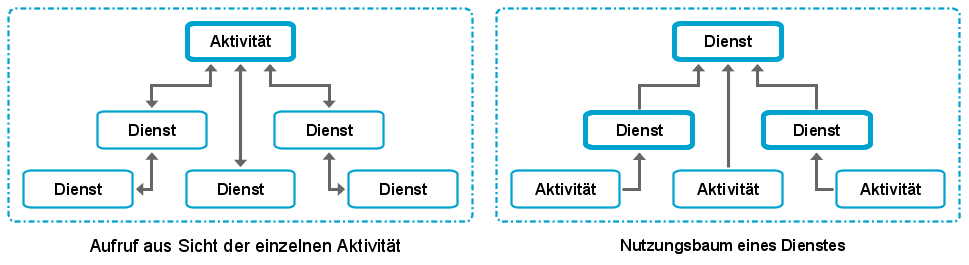
\includegraphics[width=\textwidth]{img/Serviceaufbau.png}	
    \caption[Nutzung eines Dienstes]
    {Nutzung eines Dienstes  \protect\footnotemark}
    \label{fig:Nutzung eines Dienstes}
\end{figure}
\footnotetext{in Anlehnung an \citeauthor{Masak.2007} \citeyear{Masak.2007} \cite{Masak.2007} }

Hierbei wird die wesentliche Geschäftslogik der Aktivitäten in digitalen Diensten gekapselt, während der übergreifende Geschäftsprozess in Form von Anwendungssoftware die eher reaktive und demnach dynamische Ausführungssemantik implementiert. 
\cite{Teusch.2016}
Unter dem Aspekt der Wiederverwendbarkeit eines Dienstes in einer \ac{SOA} sollte des Weiteren der in Abbildung \ref{fig:Nutzung eines Dienstes} illustrierte Umstand, dass digitale Dienste zur Ausführung einer Aktivität auf Basis weiterer Dienste aufgebaut sein können oder im Umkehrschluss ein Dienst von unterschiedlichen Aktivitäten genutzt werden kann, einer kritischen Betrachtung unterzogen werden.
\cite{Masak.2007}

Sogenannte Webservices stellen dabei eine auf \ac{XML} ausgerichtete und auf offenen Standards basierende Technologie zur Realisierung einer \ac{SOA} dar, indem sie die in einer beliebigen Programmiersprache implementierte Geschäftslogik in Form von Diensten anhand vereinheitlichter Schnittstellen nach außen zur Verfügung stellen.
\cite{Masak.2005}
Ein Webservice ist als Maschine-zu-Machine-Kommunikation zu betrachten. Diese Maschinen sprechen über offenen Standards miteinander. 
\cite{Finger.2009b}
Nachdem ein Webservice in ein Anwendungssystem integriert wurde, erfolgt die Kommunikation in der Regel automatisch. 
Ein Endanwender auf der Seite der Benutzerschnittstelle wird nicht zur Kenntnis nehmen, dass die Anwendungssoftware, die er bedient, mit einem Webservice kommuniziert. Dieses Prinzip entspricht ebenfalls dem Grundgedanken einer \ac{SOA}.
\cite{Teusch.2016}
Auf diese Weise können Webservices beispielsweise aus einem Geschäftsprozess heraus aufgerufen werden, ohne ihre konkrete Implementierung zu kennen, was insbesondere in einem geschäftsprozess- oder unternehmensübergreifenden Kontext ein bedeutender Faktor ist. Zur Änderung eines Geschäftsprozesses bedarf es lediglich einer Anpassung der Ausführungssemantik der Anwendungssoftware durch veränderte Aufrufe von bestehenden oder zusätzlichen Webservices. 

\todo{SOA Texte durch SAP Book Quelle ersetzen \cite{Pohl.2009} \cite{Hoppe.2011}}
% \begin{attentionForm}[SOA und Webservices nicht grundsätzlich synonym]
% An dieser Stelle sei jedoch der Hinweis erlaubt, dass das Konzept der Serviceorientierung allgemeiner ist und schon früher existierte als Webservices. Webservices sollten daher nur als eine, wenn auch zum Verfassungszeitpunkt dieses Buches als wahrscheinlich am besten geeignete Möglichkeit zur Realisierung serviceorientierter Architekturen betrachtet werden.
% \end{attentionForm}

Ferner können auch von Menschen ausgeführte Aktivitäten als Dienste gekapselt und mit Benutzerschnittstellen ausgestattet werden, indem die Aufforderung zum Beginn der manuellen Aktivität durch eine geeignete Ausgabe signalisiert wird, woraufhin der erfolgreiche Abschluss der manuellen Aktivität oder ein erforderlicher Abbruch wiederum durch eine Eingabe quittiert wird. 
Auf diese Weise ist auch die Integration manueller Aktivitäten in einen automatisierten Geschäftsprozess möglich.
\cite{Weske.2007}

Für die Konzeption und Implementierung von automatisierbaren Geschäftsprozessen ist eine angemessene Spezifizierung erforderlich, die verschiedene Kriterien erfüllen muss.
Bei der Betrachtung dynamischer Geschäftsprozesse im Rahmen dieser Bachelorarbeit spielen dabei auch solche Merkmale eine herausragende Rolle, welche die Ausprägung dynamischer Eigenschaften anhand einer zielgerichteten Ereignisorientierung und Ereignisverarbeitung unterstützen. 

Im Fokus der Betrachtungen sind verschiedene Kriterien zur Auswahl einer geeigneten Modellierungssprache für das zugrunde liegende Geschäftsprozessmodell von Belang, die in Tabelle \ref{tab:Kriterien für Modellierungssprachen} jeweils mit einer Beschreibung ihrer Bedeutung aufgeführt sind.

\begin{table}[H]
	\centering
	\begin{tabularx}{\textwidth}{l X} 
		\toprule
		\textbf{Kriterium}  &   
		\textbf{Beschreibung}  \\ 
		\toprule
		Funktionalität &   
		Unterstützung verschiedener Aktivitätsarten, die Darstellung sequenzieller, paralleler, alternativer und iterativer Prozessabläufe sowie die Verbindung von Aktivitäten mit Objekten, Relationen und Rollen. \cite{Funk.2010b} \\  \cmidrule(r){1-1} \cmidrule(r){2-2}
		
		Verständlichkeit &   
		Auf fachlicher Modellebene ist eine modellbasierte Darstellung der Geschäftsprozesse erwünscht, die von Fachleuten mit betriebswirtschaftlichem und technischem Hintergrund mit vertretbarem Aufwand verstanden werden kann. \\ \cmidrule(r){1-1} \cmidrule(r){2-2}
		
		Formalisierbarkeit &   
		Die Notation soll formale oder semiformale Modellierungsregeln aufweisen, damit die Konzeption korrekter Geschäftsprozessmodelle unterstützt wird und eine nahtlose Implementierung des technischen Geschäftsprozessmodells erfolgen kann. \cite{Becker.2012}  \\ \cmidrule(r){1-1} \cmidrule(r){2-2}
		
		Unterstützung von \ac{SOA} &   
		Digitale Dienste, insbesondere Webservices, und von Menschen durchgeführte Aktivitäten mit geeigneten Benutzerschnittstellen sollen integriert werden können.  \\ \cmidrule(r){1-1} \cmidrule(r){2-2}
		
		Ereignisverarbeitung &   
		Die Modellierungssprache soll ein Konzept für die Integration von Ereignissen in das Geschäftsprozessmodell enthalten und insgesamt eine hohe Ereignisorientierung aufweisen.   \\ \cmidrule(r){1-1} \cmidrule(r){2-2}
		
		Standardisierung &   
		Die Modellierungssprache soll durch eine zentrale Institution standardisiert worden sein oder zumindest einen anerkannten Industriestandard darstellen. \\ \cmidrule(r){1-1} \cmidrule(r){2-2}
		
		Werkzeugunterstützung &   
		Umfangreiche Softwarewerkzeuge für die Modellierung sollen verfügbar sein.  \\
	    \bottomrule
	\end{tabularx}
	\caption[Kriterien für Modellierungssprachen]
    {Kriterien für Modellierungssprachen für dynamische Geschäftsprozesse}
    \label{tab:Kriterien für Modellierungssprachen}
\end{table}

\subsection{Gegenüberstellung geeigneter Modellierungssprachen}
Im Folgenden werden bekannte und etablierte Modellierungssprachen für die Modellierung von Geschäftsprozessen herangezogen, die als Basis für dynamische Geschäftsprozesse dienen können. 
Diese werden zunächst einzeln begreiflich gemacht und anschließend in Bezug auf die in Tabelle \ref{tab:Kriterien für Modellierungssprachen} genannten Kriterien in einer tabellarischen Übersicht gegenübergestellt. 
% Es ist nicht Ziel des folgenden Abschnitts die \acl{EPK}, \acl{BPMN} 2.0 und  Aktivitätsdiagramme der \acl{UML} ausführlich zu diskutieren und vollumfänglich darzustellen.
Es sollen wesentliche Eigenschaften unds Elemente daraus erklärt werden, die für das Verständnis dieser Bachelorarbeit notwendig sind.

\paragraph{\acl{EPK}}
Die \textit{\acf{EPK}} stellt die zentrale Modellierungssprache in der \acf{ARIS} dar.
Entwickelt wurde die \ac{ARIS}-Architektur bereits \citeyear{Scheer.1991} am Institut für Wirtschaftsinformatik in Zusammenarbeit mit dem \ac{CIM}-Technologie-Transfer-Zentrum an der Universität des Saarlandes in Kooperation mit der SAP AG.\footnote{Am 07. Juli 2014 erfolgte eine Umwandlung der SAP AG von einer Aktiengesellschaft in eine Europäische Aktiengesellschaft (SE).}
\cite{Scheer.1991}
Der Modellierungsansatz der \ac{EPK} hat sich insbesondere im deutschsprachigen Raum als eine der meistverbreitetste semiformale Methode zur Modellierung von Geschäftsprozessen durchgesetzt. 
\cite{Gadatsch.2013}
Diese Verbreitung lässt sich unter anderem darauf zurückzuführen, dass die SAP SE die \ac{EPK} als Standard in ihr Produktportfolio integriert hat. 
\cite{Staud.2006}
In \ac{EPK}s, die nicht sequentiell ablaufen, bilden Konnektoren die Verknüpfungsknoten. Gemeint sind hierbei die aus der Aussagenlogik stammenden konjunktiven, adjunktiven und disjunktiven Verknüfungen. Dadurch wird gewährleistet, dass auch alternative, parallele und iterative Geschäftsprozessabläufe durch logische Ereignisverknüpfungen erstellt werden können.
\cite{Lehmann.2008}

In einer erweiterten \ac{EPK} wird die einfache \ac{EPK}, die sich auf Ereignisse, Funktionen, Prozessschnittstellen, Konnektoren und Kanten beschränkt, um zusätzlich verschiedene Elemente wie die organisatorische Einheit, Informationsobjekte, Anwendungssysteme oder Prozesswegweiser ergänzt. 
\cite{Seidlmeier.2015}
Dadurch ist es möglich umfassende Geschäftsprozessmodelle mit all ihren Beziehungen zum Umfeld des Geschäftsprozesses in semiformaler Form darzustellen, um durch die Modellierungssprache alle Perspektiven auf den Geschäftsprozess miteinander zu verbinden.
\cite{Gadatsch.2013}

\paragraph{\acl{BPMN} 2.0}
Die \textit{\acf{BPMN} 2.0} ist eine weltweit verbreiteter Standard der \ac{OMG} zur Modellierung von Geschäftsprozessen.
Da der ersten Version von \ac{BPMN} kein Metamodell zugrunde liegt, handelt es sich bei \ac{BPMN} in seiner ursprünglichen Gestalt streng genommen nicht um eine Modellierungssprache, dies wurde  mit Version 2.0 jedoch behoben. 
\cite{OMG.2014}

Die \ac{BPMN} 2.0 beinhaltet eine Reihe an Elementen für verschiedene Aktivitäten in einem Geschäftsprozess, wie etwa Sendeaufgaben, Empfangsaufgaben, Benutzeraufgaben, Dienstaufgaben, oder Geschäftsregelaufgaben, und eine Vielzahl an unterschiedlichen Ereignistypen, wie etwa Nachrichten-, Zeit-, Signal- oder Fehlerereignisse. 
Darüber hinaus kann der Ablauf eines Prozesses mithilfe sogenannter Gateways gesteuert werden und es kann zudem auf Datenobjekte zugegriffen werden. 
\cite{Weidlich.2010}
Obwohl die Geschäftsprozessmodellierung in \ac{BPMN} 2.0 bezüglich der konkreten Realisierungstechnologien allgemein gehalten ist, werden \ac{SOA} und Webservices durch die reichhaltige Auswahl an Elementen in besonderem Maße unterstützt.
\cite{Jobst.2010}

\paragraph{Aktivitätsdiagramme der \acl{UML}}
Das Aktivitätsdiagramm ist ein Diagrammtyp, der von der \ac{OMG} sowie der \ac{ISO} zusammen mit anderen Diagrammtypen zur Modellierung von Informationen in der \acf{UML} vereinheitlicht wurde.
\cite{OMG.2014}\cite{ISO.2012}
\ac{UML} ist heute eine der dominiernden Modellierungssprachen zur Darstellung informationstechnischer und anderer Systeme, die sich bereits in vielfältigen Einsatzgebieten in der Praxis bewährt hat.
Neben einer grafischen Notation spezifiziert die \ac{UML} auch die Semantik objektorientierter Komponenten und deren Beziehungen mit definierten Regeln für Strukturen und Abläufe.
\cite{Rumpe.2011}

Obwohl die \ac{UML} ursprünglich nicht für die Modellierung von Geschäftsprozessen entworfen wurde, ist eine Geschäftsprozessmodellierung dennoch durch den Entwurf von Aktivitätsdiagrammen eingeschränkt möglich, da hiermit funktionale Abläufe mit Hilfe von Aktivitäten und Verknüpfungen darstellbar sind. 
\cite{vanRanden.2016}
Wohl aber existieren verschiedene Defizite, etwa bezüglich der Verarbeitung von Ereignissen oder durch eine umständliche Darstellung komplexer Verknüpfungen, da bei der \ac{UML} die Systemorientierung gegenüber der Geschäftsprozessorientierung deutlich prädominiert.
\cite{Staud.2006}

\paragraph{Gegenüberstellung der Modellierungssprachen}
In Tabelle \ref{tab:Bewertung von Modellierungssprachen} wird die Eignung der vorgestellten Modellierungssprachen in Bezug auf die relevanten Kriterien aus dem vorherigen Abschnitt in tabellarischer Form gegenübergestellt.

\newcolumntype{Y}{>{\centering\arraybackslash}X}
\begin{table}[H]
	\centering
	\begin{tabularx}{\textwidth}{l Y Y Y} 
		\toprule
		\textbf{Kriterium}  &   
	    \multicolumn{3}{c}{\textbf{Modellierungssprache}}	  \\   \cmidrule(r){2-4}
	    
	                  &   
		\textbf{\acs{EPK}}\cite{Scheer.1991}\cite{Lehmann.2008}      &
		\textbf{\acs{BPMN}}\cite{OMG.2014}\cite{Weidlich.2010}       &
		\textbf{\acs{UML}}\cite{ISO.2012}\cite{Rumpe.2011}	    \\  \cmidrule(r){1-1} \cmidrule(r){2-2} \cmidrule(r){3-3} \cmidrule(r){4-4}
	    
		Funktionalität &   
		\CIRCLE  &
		\CIRCLE   &
		\CIRCLE		\\ \cmidrule(r){1-1} \cmidrule(r){2-2} \cmidrule(r){3-3} \cmidrule(r){4-4}
		
		Verständlichkeit &   
		\CIRCLE &
		\CIRCLE   &
		\LEFTcircle			\\ \cmidrule(r){1-1} \cmidrule(r){2-2} \cmidrule(r){3-3} \cmidrule(r){4-4}
		
		Formalisierbarkeit &   
		\LEFTcircle	 &
		\CIRCLE   &
		\CIRCLE		\\ \cmidrule(r){1-1} \cmidrule(r){2-2} \cmidrule(r){3-3} \cmidrule(r){4-4}
		
		Unterstützung von \ac{SOA} &   
		\Circle &
		\CIRCLE   &
		\Circle		\\ \cmidrule(r){1-1} \cmidrule(r){2-2} \cmidrule(r){3-3} \cmidrule(r){4-4}
		
		Ereignisverarbeitung &   
		\CIRCLE &
		\CIRCLE   &
		\LEFTcircle	\\ \cmidrule(r){1-1} \cmidrule(r){2-2} \cmidrule(r){3-3} \cmidrule(r){4-4}
		
		Standardisierung &   
		\LEFTcircle	 &
		\CIRCLE   &
		\CIRCLE		\\ \cmidrule(r){1-1} \cmidrule(r){2-2} \cmidrule(r){3-3} \cmidrule(r){4-4}
		
		Werkzeugunterstützung  &
		\CIRCLE &
		\CIRCLE   &
		\CIRCLE		\\ 
	    \bottomrule
	    \multicolumn{4}{c}{
	    Legende:
	    \CIRCLE
	    erfüllt
	    \LEFTcircle
	    bedingt erfüllt
	    \Circle wenig bis nicht erfüllt}
	\end{tabularx}
	\caption[Bewertung von Modellierungssprachen]
    {Bewertung von Modellierungssprachen für dynamische Geschäftsprozesse}
    \label{tab:Bewertung von Modellierungssprachen}
\end{table}

Es wird ersichtlich, dass für die Spezifizierung dynamischer Geschäftsprozessmodelle zwar alle Modellierungssprachen durch Werkzeugunterstützung praktisch anwendbar sind, diese sich allerdings deutlich anhand anderer Kriterien unterscheiden. Auffallend ist des Weiteren, dass die Unterstützung der benötigten Funktionalitäten in allen betrachteten Modellierungssprachen gegeben ist, sodass grundsätzlich die Schlussfolgerung gezogen werden kann, dass alle Modellierungssprachen prinzipiell für die Modellierung dynamischer Geschäftsprozesse einsetzbar sind. 

Aufgrund der zwingenden Ereignisbehandlung des Geschäftsprozessmodells, um für die notwendige Dynamik des Geschäftsprozesses zu sorgen, werden lediglich \ac{EPK} und \ac{BPMN} 2.0 als Modellierungssprachen in Betracht gezogen. 
\ac{BPMN} 2.0 zeichnet sich hierbei durch die erforderliche Untersützung von SOA mit Webservices und eine bessere Ausgestaltung der Ereignisverarbeitung mit umfassenderen Ereigniskonzepten sowie einer unabhängig regulierten Standardisierung aus. Letzteres drückt sich insbesondere in der Möglichkeit der grafischen Modellierung von Geschäftsprozessen und somit einer besseren Modellkonsistenz auf der fachlichen Ebene aus. Aus diesen Gründen fällt die Wahl schließlich auf den Einsatz von \ac{BPMN} 2.0 zur formalen Beschreibung des Geschäftsprozessmodells in Kapitel \ref{ch:Durchfuehrung}. 

\section{Konzept der Ereignisverarbeitung}\label{sec:Ereignisverarbeitung}
In der realen Welt ist eine Wechselwirkung aller Geschehnisse mit einer Vielzahl von divergenten, meist nicht-deterministisch eintretenden Ereignissen zu beobachten, als Konsequenz folgt eine signifikante Beeinflussung auf den Fortgang der Geschehnisse.
\cite{Grauer.2010}
Dieser Tatbestand findet sich auch in den Abläufen und Geschäftsprozessen in Unternehmen wieder.
Ein Unternehmen ist demzufolge gezwungen, auf diese Ereignisse angemessen und möglichst zeitnah zu reagieren – die Unternehmen operieren demnach ereignisgesteuert. 
\cite{Schaaf.2015}
Mit dem Konzept der Ereignisverarbeitung rücken Ereignisse als zentraler Leitgedanke einer Orientierung an Ereignissen in den Fokus der Gestaltung von Geschäftsprozessen, indem Ereignisse als Baustein der Softwarearchitektur und der Geschäftslogik in den Mittelpunkt der Betrachtung rücken. 
\cite{Bruns.2010}

Die resultierenden ereignisgesteuerten Unternehmensanwendungen ermöglichen eine praxisnahe Darstellung der dynamischen Geschäftsprozesse eines Unternehmens. 
Das Ziel ist es dadurch die Agilität, Reaktionsfähigkeit und Echtzeitfähigkeit der Geschäftsprozesse eines Unternehmens zu erhöhen. 
In der Praxis hat eine derartige Ereignisorientierung in Unternehmensanwendungen bereits breiten Zuspruch gefunden. 
\cite{Bruns.2015}
In diesem Kontext beruhen ereignisgesteuerte Architekturen, englisch \ac{EDA}, auf einem ereignisgesteuerten Prinzip, bei dem eine lose Kopplung zwischen den beteiligten Komponenten eines Informationssystems vorgesehen ist.  
In ihrer reinen Ausprägung kommunizieren diese Komponenten ausschließlich mittels sogenannter Ereignisbenachrichtigungen, englisch \textit{Event Messages}, miteinander.
Abbildung \ref{fig:Grundschritte von ereignisgesteuerten Architekturen} illustriert den Ablauf der Grundschritte ereignisgesteuerter Architekturen, deren Charakteristika nachfolgend erläutert werden.
\cite{Schaaf.2015}

\begin{figure}[H]
	\centering 
    \begin{tikzpicture}
        \fill[even odd rule, white] circle (1.5);
    
       \node at (0,0) [
          font  = \sffamily\Large\bfseries\color{black!85},
          align = center
       ]{
          \acs{EDA}
       };
       \arcarrow{197}{ 96}{Erkennen}
       \arcarrow{ 89}{-17}{Verarbeiten}
       \arcarrow{199}{341}{Reagieren}
    \end{tikzpicture}
    \caption[Grundschritte von ereignisgesteuerten Architekturen]
    {Grundschritte von ereignisgesteuerten Architekturen \protect\footnotemark}
    \label{fig:Grundschritte von ereignisgesteuerten Architekturen}
\end{figure}
\footnotetext{in Anlehnung an \citeauthor{Bruns.2010} \citeyear{Bruns.2010} \cite{Bruns.2010} }

Demnach besteht eine zentrale Charakteristik von ereignisgesteuerten Architekturen aus der Komposition von drei Grundschritten: \textit{Erkennen, Verarbeiten und Reagieren von oder auf Ereignisse.}

\paragraph{Erkennen} 
Das Auftreten von relevanten Informationen und Sachverhalten in  den Geschäftsprozessen ist der Ausgangspunkt für die Erkennung von Ereignissen.
Diese Informationen und Sachverhalte werden analysiert, als Ereignisse klassifiziert und spiegeln einen spezifizierten Ausschnitt des Zustands eines Geschäftsprozesses wieder. 
Für registrierte Ereignisse wird ein entsprechendes Ereignisobjekt generiert.
Entscheidend für ereignisgesteuerte Informationssysteme ist, dass die Ereignisse unmittelbar zum Zeitpunkt ihres Auftretens erkannt werden und nicht zeitverzögert.
\cite{Bruns.2010}

\paragraph{Verarbeiten}
Im Verarbeitungsschritt werden die erkannten Ereignisse, die aus unterschiedlichen Ereignisquellen stammen können, analysiert. Bei der Analyse werden Ereignisse zu Einheiten aggregiert, mit anderen Ereignissen verknüft, generalisiert, aufgeteilt oder aber auch als irrelevant eingestuft. 
Gesucht werden Paradigmen in den gesammelten Ereignissen, die bestimmte Beziehungen und Abhängigkeiten zwischen den Ereignissen ausdrücken.
\cite{Hedtstuck.2017}

\paragraph{Reagieren}
Aufgrund von analysierten Mustern, die im Fluss der eingetretenen Ereignisse erkannt wurden, können vielfältige Arten von Reaktionen zeitnah veranlasst werden. 
Die Reaktionen, die angestrebt werden, charkterisieren sich durch Aktualität und Individualität, wie etwa die unmittelbare Übergabe der Ereignisse an Anwendungssysteme, das Senden von Benachrichtigungen, der Aufruf von Funktionen in Form von digitalen Diensten, das Auslösen eines Geschäftsprozesses oder die Initiierung von manuellen Aktivitäten durch menschliche Benutzer, aber auch die Generierung neuer Ereignisse ist eine legitime Reaktion.
\cite{Bruns.2010}

In der Realität existieren allerdings kaum Geschäftsprozesse, bei denen eine ausschließliche Kommunikation mithilfe von Ereignissen und alleinig im Rahmen der beschriebenen Grundschritte einer \ac{EDA} erfolgen, weshalb auch Anwendungen mit teilweiser Ereignisverarbeitung und partieller Anwendung dieser Grundschritte die Umsetzung einer ereignisgesteuerten Architektur zugeschrieben.
\cite{Etzion.2011}
Die \ac{SOA}-Architektur beinhaltet, wie in Abschnitt \ref{sec:Automatisierung} beschrieben, die Konzepte, die notwendig sind, um Echtzeit-Anwendungssysteme zu ermöglichen und die Unterstützung der Dynamik ereignisgesteuerter Geschäftsprozesse zur selben Zeit zu gewährleisten, nicht vollständig.
Eine \ac{SOA} ohne Ereignisverarbeitung ist folglich nicht in der Lage, den aktuellen Zustand von Aktivitäten zu erkennen, da hierzu in Echtzeit temporale und kausale Verbindungen zwischen Geschäftsprozessen und Aktivitäten identifiziert und analysiert werden müssen. 
Eine \ac{EDA} kann als Maßnahme auch eine \ac{SOA} komplementieren, zumal beide Konzepte grundsätzlich modulare und verteilte Informationssysteme mit loser Kopplung unterstützen, um die Vorteile beider Architekturen im Kollektiv zu nutzen. 
Für eine derartige Kombination von \ac{SOA} und \ac{EDA} wird häufig die Bezeichnung Event-Driven SOA genutzt.
In dieser Ausprägung können Ereignisse den Aufruf von digitalen Diensten auslösen, woraufhin im Verlauf, deren Ausführung weitere Ereignisse generiert werden, die parallel von einem Ereignisverarbeitungsdienst analysiert und verarbeitet werden. 
\cite{Bruns.2010}

Im Zusammenhang mit der Ereignisverarbeitung in Unternehmensanwendungen wird der Begriff Echtzeit, englisch real-time, häufig verwendet, um die Aktualität von verarbeiteten Ereignissen zu hervorzuheben.
\cite{Bruns.2015}
Echtzeit wird jedoch nicht im Sinne der Informatik verstanden, wonach für jede Funktion die exakte Einhaltung einer restriktiv vorgeschriebenen Antwortzeit erforderlich ist, um die Gegenwartsbezogenheit und Vorhersagbarkeit von Informationssystemen sicherzustellen.
Vielmehr dominiert ein betriebswirtschaftliches Verständnis, das darauf Bedacht ist, in allen relevanten Informationssystemen aktuelle Informationen bereitzustellen, ohne spezifizierte Leistungskennzahlen zur Erfüllung von Echtzeit zu formulieren.
\cite{Worn.2005}
Unter Echtzeit versteht man aus dieser Sicht daher die möglichst zeitnahe Verfügbarkeit, Transparenz und Nutzbarkeit von Informationen ohne unnötige Zeitverzögerung.
Eingehende Ereignisse werden somit im Rahmen der Ereignisverarbeitung analysiert, sobald sie auftreten, um geeignete Reaktionen in Echtzeit auslösen zu können.
\cite{Grauer.2010}

\subsection{Merkmale und Kriterien}
Die \ac{EDA} wird, wie schon erwähnt, im Wesentlichen durch die drei Grundschritte Erkennen, Verarbeiten und Reagieren charakterisiert, woraus sich drei logische architektonische Schichten für eine Ereignisverarbeitung ergeben: Ereignisquellen, Ereignisverarbeitung und Ereignisbehandlung. Das
Zusammenspiel dieser drei Schichten wird  in Abbildung \ref{fig:Grundlegender architektonischer Entwurf einer EDA} veranschaulicht.

\begin{figure}[H]
	\centering 
    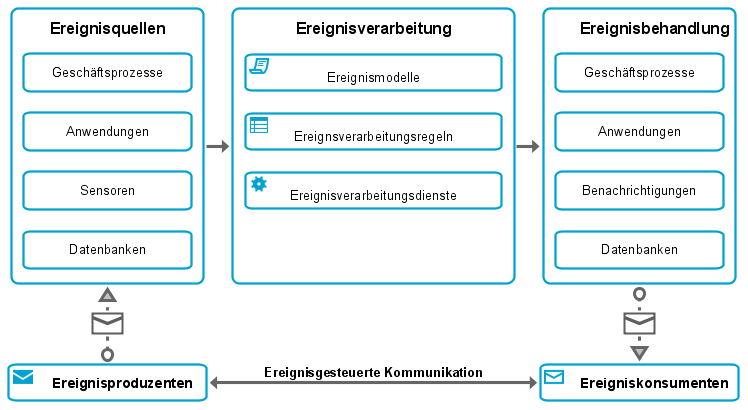
\includegraphics[width=\textwidth]{img/Ereignisverarbitungablauf.png}	
    \caption[Grundlegender architektonischer Entwurf einer EDA]
    {Grundlegender architektonischer Entwurf einer EDA}
    \label{fig:Grundlegender architektonischer Entwurf einer EDA}
\end{figure}
\footnotetext{in Anlehnung an \citeauthor{Metz.2014} \citeyear{Metz.2014} \cite{Metz.2014} }

\todo{abbildung erkären}

\todo{Formulierung der Ereignisverarbeitungsregeln}

\missingfigure{Kriterien für Funktionalitäten der Ereignisverarbeitung}

\subsection{Bewertung von Funktionalitäten der Ereignisverarbeitung}

\todo{Referenzieren auf \cite{Vidackovic.2010}}

\missingfigure{Tabelle  Bewertung von Funktionalitäten der Ereignisverarbeitung}


\section{Dynamische Geschäftsprozesse auf Basis von Ereignisverarbeitung}\label{sec:Kombi}
Bei der Automatisierung von dynamischen Geschäftsprozessen wächst die Notwendigkeit, auf kritische Ereignisse in Echtzeit und ohne Latenzzeiten zu reagieren. 
Die Integration von Ereignisverarbeitungskonzepten in die Konzeption dynamischer Geschäftsprozesse ist ein geeignetes Mittel, um den steigenden Anforderungen an das Echtzeit-Management von Geschäftsprozessen unter Berücksichtigung relevanter Ereignisse zur Laufzeit gerecht zu werden. 
\cite{Abolhassan.2016}
Die Vorteile für ein Unternehmen bei einer solchen Vervollständigung der Geschäftsprozessautomatisierung mit Konzepten der Ereignisverarbeitung gründen sich im Wesentlichen auf die folgenden Merkmale:

\begin{itemize}
    \item 
    Identifizierung relevanter oder kritischer Situationen für den Geschäftsprozess unter Berücksichtigung externer Ereignisse aus dem Geschäftsumfeld und interner Ereignisse aus dem Geschäftsprozess.
    \item 
    Möglichkeit der unmittelbaren Reaktion auf veränderliche Situationen durch Verarbeitung von Ereignissen in Echtzeit.
    \item
    Möglichkeit der Trennung der Ereignisverarbeitungslogik von der Geschäftsprozesslogik durch lose Kopplung und Kommunikation über Ereignisobjekte.Automatisierte Adaptionen von Geschäftsprozessen auf Basis von aktuellen Ereignissen.
    \item
    Gute Unterstützung von verteilten Umgebungen, die insbesondere in unternehmensübergreifenden Geschäftsprozessnetzwerken und \ac{SOA}-Umgebungen eine bedeutende Rolle spielen.
\end{itemize}

Es existieren bereits erste Forschungsansätze mit dem Ziel der Anreicherung von Geschäftsprozessmodellen mit Konzepten der Ereignisverarbeitung, die unter der englischen Bezeichnung Event-Driven Business Process Management zusammengefasst werden. Ausgewählte Konzepte aus diesem Bereich werden im Folgenden vorgestellt und anschließend anhand wesentlicher Kriterien gegenübergestellt.

\subsection{Merkmale und Kriterien}

Dynamische und somit ereignisorientierte Geschäftsprozesse operieren prinzipiell auf zwei Ebenen, der Geschäftsprozessebene und der Ereignisverarbeitungsebene. 
Diese erfüllen ihre Aufgaben in erster Linie separat und in paralleler Weise, kommunizieren allerdings mittels des Austauschs von Ereignissen miteinander, was in diesem Kontext den maßgeblichen Aspekt darstellt. 
Abbildung \ref{fig:Ebenen dynamischer Geschäftsprozesse} illustriert in schematischer Darstellung die Zusammenhänge.

\begin{figure}[H]
	\centering 
    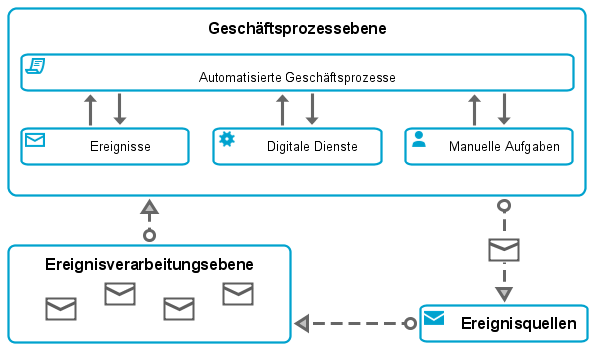
\includegraphics[width=\textwidth]{img/dynamicbp.png}	
    \caption[Ebenen dynamischer Geschäftsprozesse]
    {Ebenen dynamischer Geschäftsprozesse \protect\footnotemark}
    \label{fig:Ebenen dynamischer Geschäftsprozesse}
\end{figure}
\footnotetext{Eigene Darstellung, in Anlehnung an \citeauthor{Vidackovic.2014} \citeyear{Vidackovic.2014} \cite{Vidackovic.2014} }
\footnotetext{Die Abbildung dient lediglich der Visualisierung und ist nicht \ac{BPMN} 2.0 konform.}

Auf der Ereignisverarbeitungsebene werden eingehende Ereignisse aus diversen externen und internen Ereignisquellen kontinuierlich analysiert, wobei zudem Ereignisse generiert werden können, welche wiederum dieselbe Analyse durchlaufen. 
Da zwischen der Ereignisverarbeitungsebene und der Geschäftsprozessebene mit Ereignissen kommuniziert werden kann, können diese generierten Ereignisse als unmittelbare Reaktion eine dynamische Wirkung auf den Ablauf des laufenden Geschäftsprozess ausüben.
Der Geschäftsprozess fungiert demnach einerseits als eine der internen Ereignisquellen für die Ereignisverarbeitungsebene und andererseits als wesentlicher Ereigniskonsument der generierten Ereignisse zur Adaption des Prozessablaufs.
\cite{Benker.2016}

Auf der Geschäftsprozessebene erfolgt der operative und automatisierte Ablauf von Aktivitäten des Geschäftsprozesses, wobei Letztere in einer \ac{SOA} überwiegend auf elektronischen Diensten basieren, die als Webservices über standardisierte Schnittstellen aufgerufen werden und auch über Unternehmensgrenzen hinweg verteilt sein können.
\cite{Finger.2009}
Bei den Aktivitäten kann es sich darüber hinaus auch um manuelle Benutzeraufgaben handeln, die zwar von Menschen ausgeführt werden, aber dennoch mittels informationstechnischen Schnittstellen in einen automatisierten Prozessablauf integriert werden können.
\cite{Bruns.2010}


In ereignisorientierten im Gegensatz zu ablauforientierten Geschäftsprozessen üben Ereignisse zur Laufzeit einen signifikanten Einfluss auf den Prozessablauf aus, sodass die Geschäftsprozesse anhand geeigneter Ereignisverarbeitungsregeln mit dynamischen Eigenschaften ausgestattet werden können. 

\subsection{Gegenüberstellung vorhandener Forschungsansätze}
Die wesentlichen Aspekte der existierenden Forschungsansätze werden zunächst einzeln betrachtet und anschließend gegenübergestellt.

\paragraph{Entwicklung agiler Geschäftsprozesse mit Ereignisverarbeitung}
Dieser Forschungsansatz von \citeauthor{Alexopoulou.2008} aus dem Jahr \citeyear{Alexopoulou.2008} liefert eine Vorgehensweise zur Entwicklung dynamischer und ereignisgesteuerter Geschäftsprozesse, die nicht in Form eines abgeschlossenen Systems modelliert werden, sondern lediglich aus einzelnen Ereignis-Aktivität-Einheiten, sogenannten Dynamikeinheiten, bestehen. 
\cite{Alexopoulou.2008} 
Diese werden in Echtzeit auf der Ereignisverabreitungsebene ausgeführt und fügen den Geschäftsprozess dynamisch zusammen, wobei neue Ereignis-Aktivität-Einheiten bedarfsgerecht hinzugefügt werden können. 

Ein Defizit dieses Forschungsansatzes ist die fehlende Betrachtung des gesamten Ablaufs. Das Konzept dieser Dynamikeinheiten wird auch in dieser Bachelorarbeiten aufgegriffen, allerdings ausgehend von einem in seiner Gesamtheit modellierten Geschäftsprozess, der in diese Einheiten zerlegt wird.

\paragraph{RESTful SOA zur Automatisierung von Geschäftsprozessen}
Die Realisierung von \ac{SOA} in diesem Forschungsansatz von \citeauthor{Wolf.2016} ist in Übereinstimmung mit den Prinzipien von \ac{REST}. 
\footnote{
Da der technische Fokus in dieser Arbeit auf der Geschäftsprozessebene liegt, werden die einzelnen technischen Konzepte an dieser Stelle nicht weiter vertieft.
Für eine detaillierte Betrachtung der Prinzipien von \ac{REST} sei lediglich auf weiterführende Literatur verwiesen.
\cite{Wolf.2016}\cite{Masak.2007}\cite{Finger.2009}}
Die \ac{REST}ful \ac{SOA} entsteht durch den Entwurf serviceorientierter Architekturen gemäß den Bedingungen und Technologien von \ac{REST}. \ac{REST} ist ein Architekturstil für die Gestaltung verteilter Systeme, insbesondere bei der Umsetzung von Webservices. Durch dieses Vorgehen wird auf eine modellbasierte Spezifikation von \ac{REST}ful \ac{SOA} für die Automatisierung von Geschäftsprozessen abgezielt. \cite{Wolf.2016}

Insbesondere die Überwindung der semantischen Lücke zwischen Geschäftsprozessmodell und Anwendungssystem durch ein systematisches Vorgehen wird in diesem Forschungsansatz behandelt. Die identifizierten Probleme werden durch einen Ansatz zur Konzeption eines Anwendungssystems auf Basis von auf fachlicher Ebene modellierten Geschäftsprozessen angegangen.  
Es fehlen allerdings Möglichkeiten zur Modellierung wesentlicher Konzepte der Echtzeitverarbeitung von Ereignissen.
Da der Forschungsansatz wohl aber auf die automatisierte Ausführung von Geschäftsprozessen mithilfe von digitalen Diensten ausgerichtet ist, bleibt der Ansatz für die softwaretechnische Implementierung in Kapitel von Relevanz. 

\paragraph{Methodology for Business Dynamics\textsuperscript{dbpm}}
Der Forschungsansatz von \citeauthor{Vidackovic.2014} stellt die  Methode [moby]\textsuperscript{dbpm} zur Entwicklung dynamischer Geschäftsprozesse mit Ereignisverarbeitung dar. Der Name [moby]\textsuperscript{dbpm} steht dabei für Methodology for Business Dynamics und dbpm für Dynamic Business Process Management. Der Ansatz bietet einen geeigneten Lösungsansatz für die Problemstellung dynamischer Geschäftsprozesse mit Ereignisverabeitung an und stellt das dafür benötigte, webbasierte Modellierungswerkzeug zur Verfügung. 
\cite{Vidackovic.2014}

Die Modellierung wird in einer von \citeauthor{Vidackovic.2014} erweiterten Form von \ac{BPMN} 2.0 vorgenommen. Des Weiteren folgt der Ansatz den Konzepten der modellbasierten Softwarentwicklung. Die Geschäftsprozessmodelle können in Kombination mit dem Produkt \textit{Esper} mit Code angereichert und anschließend automatisch ausgeführt werden ohne eine weitere Implementierung in ein Anwendungssystem. Der Ansatz einer modellbasierten Softwarentwicklung wird im Rahmen dieser Bachelorarbeit, aufgrund mangelnder Integrationsmöglichkeiten mit SAP S/4HANA Cloud, nicht weiter verfolgt. Die Ergebnisse des Forschungsansatzes von \citeauthor{Vidackovic.2014} werden jedoch als wertvoller Beitrag in diesem Fachbereich angesehen.  

\paragraph{SOEDA-Methode}
SOEDA beschreibt ein Verfahren zur Entwicklung von Anwendungssystemen durch die Zusammenführung von serviceorientierten (SOA) und ereignisgesteuerten Architekturen (EDA). Geschäftsprozesse werden hier mit \ac{EPK}s modelliert. 
\cite{MatthiasWieland.2009} 
Mit Hilfe von grafischen Modellierungswerkzeugen werden die zugrunde liegenden Aktivitäten modularisiert und mit entsprechenden Ereignissen gekoppelt, so dass ein Entwickler die Regeln der Ereignisverarbeitung anschließend in einer spezifischen Programmiersprache implementieren kann. 
\cite{Bruns.2010}

Schwächen der SOEDA-Methode sind die unzureichende Modellierung von Ereignisverarbeitungsregeln durch die Verwendung von \ac{EPK}s. 
\cite{RobraBissantz.2009}
Auch mangelt es an der Abbildung von Ereignissen im Geschäftsprozess, da Ereignisse nur als Teil des normalen Geschäftsprozessablaufs betrachtet werden. Mit der Version 2.0 verfügt die \ac{BPMN}, wie in Abschnitt \ref{sec:Automatisierung} erwähnt, nun nicht nur über eine grafische Notation, sondern auch über die Semantik der technischen Ausführung. Auf \ac{EPK}s kann demzufolge im Rahmen der Bachelorarbeit verzichtet werden, zumal eine Konsistenz des Geschäftsprozessmodells auf betriebswirtschaftlicher und technischer Ebene wünschenswert ist.

\paragraph{Gegenüberstellung der Ansätze}
Auf Basis der Darstellung der existierenden Forschungsansätze wird ersichtlich, dass die bestehenden Forschungsansätze für die Anreicherung von Geschäftsprozessmodellen mit Konzepten der Ereignisverarbeitung jeweils einen bestimmten Fokus besitzen, dessen Herausforderungen im Einzelfall ausreichend erfüllt werden. 
Eine Kopplung von Ereignissen und Aktivitäten mithilfe des Ansatzes von \citeauthor{Alexopoulou.2008}, fachliche Aspekte wie die der SOEDA-Methode, die technischen Möglichkeiten der \enquote{RESTful SOA} oder eine automatisierte Ausführung der [moby]\textsuperscript{dbpm} finden beispielsweise keine Betrachtung. 

Folglich lässt sich sagen, dass bisher noch kein Lösungsansatz mit einer ganzheitlichen und durchgängigen Vorgehensweise existiert, die eine vollständige, formale sowie fachlich orientierte Modellierung von Geschäftsprozessen mit dynamischen Eigenschaften auf Basis von Ereignisverarbeitung ermöglicht.


\section{Zusammenfassung der wesentlichen Erkenntnisse und Defizite}


\todo{Anpassen}

Resümierend sind im Wesentlichen folgende Erkenntnisse festzuhalten, die für die betrachtete Pro-
blemstellung von Relevanz sind:
\begin{itemize}
	\item This is a bullet point.
    \item This is another one.
\end{itemize}

Diesen Erkenntnissen kann durch den aktuellen Stand der Wissenschaft und Technik nicht in
reichendem Maße Rechnung getragen werden, da maßgebliche Defizite vorhanden sind:
\begin{itemize}
	\item This is a bullet point.
    \item This is another one.
\end{itemize}
\chapter{Bezugsrahmen und Anforderungen}\label{ch:Bezugsrahmen}
Der Bezugsrahmen dieser Bachelorarbeit soll einen exemplarischen Anwendungsfall zur Verfügung stellen, der sich für eine Dynamisierung von Geschäftsprozessen mittels Konzepten der Ereignisverarbeitung eignet. Hierbei handelt es sich um die ablauforientierte und somit eher statische Fertigungsdurchführung in der diskreten Fertigung, welche im Zuge ihrer \ac{IT}-gestützten Geschäftsprozessautomatisierung auf die Echtzeitverarbeitung verschiedenster Ereignisse angewiesen ist.
Um die betrachtete Problemstellung bei dynamischen Geschäftsprozessen bewältigen zu können, werden im Rahmen der Bachelorarbeit mithilfe von Experteninterviews Merkmale und Aktivitäten im Geschäftsprozess der Fertigungsdurchführung empirisch erhoben, sodass aus den korrespondierenden Informationen Kriterien für die Dynamisierung des Geschäftsprozesses mittels Konzepten der Ereignisverarbeitung aufgestellt werden können.
Anschließend werden Anforderungen sowohl auf Basis der im vorherigen Kapitel gewonnenen Erkenntnisse als auch aus den durchgeführten Experteninterviews sowie der Problemstellung heraus sondiert, um eine objektive Bewertung des konzipierten Geschäftsprozesses zu ermöglichen.
\section{Management von Betriebsdaten im Industriebetrieb}

\todo{Aufgaben im Industriebetrieb}

\missingfigure{Wertschöpfungskette}

\todo{}

\subsection{Geschäftsprozesse in der Produktionsplanung und -steuerung}

\subsection{Vorstellung der Fertigungsdurchführung in der diskreten Fertigung}

\section{Anforderungen}

\subsection{Methodisches Vorgehen zum Experteninterview}

\subsection{Charakteristika und Defizite der Fertigungsdurchführung}

\subsection{Ableitung der Anforderungen an die Fertigungsdurchführung}
\section{Anforderungen}\label{sec:anforderungen}

\todo{Welche Aufgaben müssen erledigt werden? tabellarisch lösen mit input outpu und zeitpunkt der ausführung (start, ende, jederzeit, nach xy)}

\todo{Freigabe mit Papieren digital aber auch analog}

\todo{}





\todo{Weclhe Anforderungen liegen in der Fertigungsdurchführung vor}

\todo{Anforderungen mit Bezug zur Software}

\todo{Anforderungen mit Bezug zur Problemstellung}


\chapter{Konzeption der Methode}

\section{Verfahrensweisen und wesentliche Gestaltungsprinzipien}

\subsection{Charakterisierung dynamischer Geschäftsprozesse}

\subsection{Grundlagen des Lean Managements}
\todo{Andere BPM-Methode finden (evtl. Lean Production)}

\subsection{Experimentelles Prototyping}
\todo{Andere Softwareentwicklungs-Methode finden!!}

\section{Darstellung der methodischen Vorgehensweise}

\chapter{Modellierung auf Geschäftsprozessebene}
\section{Anwendung der Lean Management Prinzipien}
\todo{Auf das gewählte Modell in Punkt 4 anpassen}
Um zu überprüfen, ob die im Rahmen dieser Arbeit angedachte Automatisierung von Testfällen möglich ist wird folgende Hypothese aufstellen: 

\textit{Vorher manuell ausgeführte Testfälle, welche Blackbox-Verfahren anwenden, lassen sich durch Eagle Drones automatisieren und weisen dabei äquivalente Ergebnisse auf}. 

Geprüft werden soll diese Hypothese für die im Rahmen dieser Arbeit zur Automatisierung bestimmten Testfälle. Für die Überprüfung der Hypothese wird angenommen, dass ein manueller Testfall automatisierbar ist, wenn er Bestandteil eines automati- sierten Tests ist. Gestützt wird dieses Annahme auf das Prinzip der schlüsselwortgetriebenen Automatisierung (siehe Kapitel 2.5.4). Auf dieser Basis soll ein komplexer Testfall entworfen werden, der möglichst viele zu automatisierende Testfälle enthält. Ist die Automatisierung dieses komplexen Testfalls im Rahmen der prototypischen Implementierung möglich, so kann die Hypothese für die inkludierten Testfälle als ve- rifiziert angesehen werden. Gelingt eine Automatisierung nicht, ist die Hypothese zu falsifizieren.

\subsection{Erarbeitung und Vorstellung geeigneter Maßnahmen}
\todo{Anforderungen in konkrete Maßnahmen umformen}

\subsection{Segmentierung und Bildung von Dynamikeinheiten}


\section{Modellierung des Geschäftsprozesses}
\todo{Grundlangen BPMN 2.0 + neues Modell}

\chapter{Konzeption des Ereignisverarbeitungsmodells}

\section{Spezifizierung des Ereignismodells}

\todo{Welche Ereignisse gibt es?}

\todo{Welche Daten braucht man?}




\section{Entwicklung des Ereignisverarbeitungsdienstes}

\todo{Wie wird kommuniziert?}

\missingfigure{Event Messaging Architecture}
\chapter{Softwaretechnische Implementierung}

\section{Transformation des Ereignisverarbeitungsmodells in ausführbaren Code}\label{sec:Transformation}

\todo{stellung nehmen was zu tun war in abap was zu tun war in java}

\subsection{Implementierte Komponenten}

\todo{ABAP Coding hier platzieren}

\todo{Java Coding hier platzieren}

\subsection{Softwarearchitektur}

\missingfigure{Architektur}

\subsection{Benutzung}

\todo{mini process flow}

\todo{JavaScript Coding hier platzieren}

\section{Technische Anbindung von Diensten und Ereignisquellen}

\subsection{Integration mit SAP S/4HANA Cloud}

\subsection{Anbindung von SAP Enterprise Messaging}

\subsection{Erweiterung durch Google Cloud Vision}
\section{Implementierung der Benutzerschnittstelle}\label{sec:frontend}

\subsection{Softwarearchitektur}

\subsection{Benutzung}
\chapter{Anwendung und Bewertung}

\section{Evaluation auf Geschäftsprozessebene}
\section{Anwendung des Ereignisverarbeitungsmodells}
\section{Bewertung der Anforderungserfüllung}
\chapter{Schlussbetrachtung}\label{ch:Ende}
\section{Bewertung der Anforderungserfüllung}
\section{Kritische Würdigung}\label{sec:Kritik}

% Die überschaubare Fallzahl an Interviews erhebt keinen Anspruch auf Repräsentativität, sondern stellt eine qualitative Forschungsstudie dar. 

% Mit den Ergebnissen der Experteninterviews sollten Informationen gesammelt, analysiert, in Beziehung gesetzt und verglichen werden, um Handlungsempfehlungen für den Einsatz von bürgerschaftlichem Engagement als Instrument der Kulturförderung durch Stiftungen formulieren und entwickeln zu können. Dafür wurden die Interviews mit Hilfe der qualitativen Inhaltsanalyse ausgewertet.

% Die gesammelten Daten behandeln nicht nur die Grundhaltung der Stiftungen sowohl zu bürgerschaftlichem Engagement und seiner Förderung allgemein, sondern auch deren persönliche Einschätzung zum Einsatz von bürgerschaftlichem Engagement in der Zukunft. Zudem wurden differenzierte Aspekte rund um das Thema befragt, die im weiteren Verlauf näher vorgestellt werden.

% Für die Interviews wurden 17 Experten aus u.a. 14 Stiftungen befragt (siehe Kapitel 1.3.3). Für die vorliegende Arbeit sollten die Experteninterviews dabei nicht nur als Ergänzung und Überprüfung von theoretischem Wissen dienen. Da bürgerschaftliches Engagement im Stiftungsbereich, wie bereits beschrieben, bislang wenig untersucht wurde, dienten die Aussagen der Experten auch dazu, neue Erkenntnisse für den Stiftungsbereich zu gewinnen, indem sie Auskunft über ihr eigenes Handlungsfeld und damit verbundene Eindrücke bzw. Erfahrungen in die Gespräche mit einbrachten. Damit wurden die Experteninterviews zu einer zusätzlichen Datenquelle neben den theoretischen Recherchen.

% Aufgrund dieser angelesenen sowie durch Tagungen und durch eigene Berufserfahrung erlangten Kompetenz konnte die offene Führung der Interviews umgesetzt werden. Die Reihenfolge des Leitfragebogens gab keinen zwingenden Ablauf der Diskussion vor. Die Offenheit in der Führungsstruktur der Interviews stellte sich als Bereicherung dar, da es leitfadengestützte Experteninterviews zulassen, im Interview flexibel auf neue Aspekte zu reagieren. In den Gesprächen konnte somit neben der Groborientierung am Fragebogen eine freie Diskussion und ein bereichernder Gedankenaustausch ermöglicht werden, was sich als hilfreich herausstellte, da aufgrund der Verschiedenartigkeit der befragten Stiftungen jedes Interview einer individuellen Anpassung des Leitfragebogens bedurfte.

% Die Auswahl der Experten für diese Dissertation fiel auf Personen mit unterschiedlichen Positionen in ihrer Stiftung bzw. Institution. Es wurde recherchiert, wer innerhalb der jeweils für den Forschungsschwerpunkt interessanten Stiftung am besten über das Forschungsthema diskutieren kann. 35 Deshalb wurden sowohl Geschäftsführer, als auch Vorstandsmitglieder und Leiter von Projekten oder Gruppen befragt, d.h. Vertreter der Stiftung bzw. Institution, die an verschiedenen Schaltstellen Verantwortung tragen.

% Der Expertenstatus wird hinsichtlich der spezifischen Fragestellung vom Forscher „verliehen“36, da der Experte durch seine besonderen Zuständigkeiten und Aufgaben, seine Erfahrung und Wissen „Insider-Kenntnisse“ zu dem Forschungsgegenstand beisteuern kann. Dadurch erspart die Methode eines Experteninterviews andere aufwendigere Explorationsphasen wie sie z.B. bei einer teilnehmenden Beobachtung oder einer Feldstudie nötig wären. Mit Experteninterviews können Forschungsprojekte kontextspezifisch untersucht werden. Zudem können Experten i.d.R. meist komplikationslos zu einer Interviewteilnahme bewegt werden.

% Gleichzeitig zeigte sich, dass die Interviewpartner bei der Beantwortung der Fragen von den Erfahrungen der Forscherin profitieren konnten, da neue Aspekte und Blickwinkel die Forschungsperspektive erweiterten.

% \begin{attentionForm}
% Laut Meuser und Nagel sind es eben oft nicht Vertreter der „obersten Ebene“ in einer Organisation, die sich als Experten eignen, sondern der Ebenen darunter, weil dort „das detaillierteste Wissen über interne Strukturen und Ereignisse vorhanden ist“. 
% Siehe: Meuser, Michael/Nagel, Ulrike: ExpertInneninterviews – vielfach erprobt, wenig bedacht, in: Bogner, Alexander et al.: Das Experteninterview. Theorie, Methode, Anwendung, Opladen 2009, S. 447. 

% Pfadenhauer, Michaela: Auf gleicher Augenhöhe, in: Bogner, Alexander et al.: Das Experteninterview. Theorie, Methode, Anwendung, Opladen 2009, S. 107.
% \end{attentionForm}

% \textbf{Auswertung durch eine qualitative Inhaltsanalyse nach Philipp Mayring}

\section{Ausblick}

\todo{Überlegen diesen Kapitel zu kürzen/streichen}

%	Literaturverzeichnis
\ihead{} % Neue Header-Definition
\printbibliography[title=Literaturverzeichnis]
\counterwithin{figure}{chapter}
\counterwithin{table}{chapter}
\counterwithin{figure}{chapter}
\counterwithin{algorithm}{chapter}


\cleardoublepage
% Der Anhang beginnt hier - jedes Kapitel wird alphabetisch aufgezählt. (Anhang A, B usw.)
\appendix
\ihead{\appendixname~\thechapter} % Neue Header-Definition

% appendix.tex einziehen
\chapter{Interviewprotokolle}\label{ah:protokolle}

\spaceparagraph{Vorwort zu den Experteninterviews}
Die folgenden Ausführungen fassen die Resultate der im Rahmen dieser Bachelorarbeit durchgeführten Experteninterviews zusammen.
Die Auswertung erfolgt summarisch und wird nicht wortwörtlich transkribiert.
Dieses Vorgehen ist mit dem wissenschaftlichen Betreuer dieser Bachelorarbeit abgestimmt.
Die Interviewpartnerinnen und -partner haben der Veröffentlichung ihres Interviews in der Audio- oder Textversion zugestimmt.
Aus datenschutzrechtlichen Gründen wurden in den folgenden Interviewprotokollen alle Namen, Unternehmen und Institutionen durch Pseudonyme ersetzt und dementsprechend gekennzeichnet.

\begin{itemize}
  \item
        \textit{Thema der Experteninterviews:} 
        Die Experteninterviews beziehen sich auf die Erhebung von in der Praxis eingesetzten Abläufe einer Fertigungsdurchführung in der diskreten Industrie im Allgemeinen sowie im SAP-Umfeld.
        Welche Faktoren in Form von Verschwendung negativ Einfluss auf den Geschäftsprozess nehmen und wie sich diese potenziell eliminieren ließen, wird im Rahmen der Experteninterviews ebenfalls eruiert.
        Im Fokus steht die Ermittlung der etablierten Aktivitäten und Hilfsmittel einer Fertigungsdurchführung, deren Merkmale und Defizite sowie die Identifikation von Alternativen.
  \item 
        \textit{Ziel der Experteninterviews:}
        Mit den Experteninterviews sollen tatsächliche Gegebenheiten einer Fertigungsdurchführung in der diskreten Industrie begreiflich gemacht werden. 
        Anhand der erarbeiteten Merkmale und Defizite werden anschließend formulierbare Optimierungspotenziale in Erfahrung gebracht.
        Diese Potenziale sollen als Summarium an Anforderungen einer Fertigungsdurchführung im SAP-Umfeld zur Verfügung stehen und als Fundament der Evaluation der zu betrachtenden Maßnahmen dienen.
\end{itemize}

\newpage
% **************************************************************************************
% * Anwenderperspektive                                                               
% **************************************************************************************
\tocless\section{Interview mit einem Branchenexperten}\label{ah:interviewTUD}

\spaceparagraph{Experte für das Experteninterview}
\textit{Prof. Dr.-Ing. Max Mustermann \footnote{Der Name \textit{Max Mustermann} repräsentiert den Namen des Branchenexperten.}} wird für das Experteninterview befragt.
Er ist Institutsleiter des Instituts für Produktionsmanagement, Technologie und Werkzeugmaschinen der \textit{Technische Universität Musterstadt \footnote{Die \textit{Technische Universität Musterstadt} repräsentiert das Bildungsinstitut des Branchenexperten.}}, in dessen Zuständigkeit die folgenden Forschungsbereiche fallen: Digitalisierung und Vernetzung von Fertigungsprozessen, Echtzeitdatenerfassung und Automatisierungstechnik für die diskrete Fertigung, Werkzeugmaschinen und Industrierobotik \footnote{Die Aufzählung der Forschungsbereiche dient lediglich als Überblick und ist nicht vollständig.}

Die Tätigkeit des Institutsleiters übt \textit{Prof. Dr.-Ing. Max Mustermann} seit dem Jahr 2019 an der \textit{Technischen Universität Musterstadt} aus. Seit dem Jahr 2002 hatte er diverse Leitungsfunktionen mit den Themenschwerpunkten Werkzeugtechnologie, Produktionsplanung, Prototypen- und Serienfertigung, Betriebsmittelkonstruktion und Automatisierungstechnik sowie Engineering und Innovationsmanagement bei der \textit{Musterberger Druckmaschinen AG \footnote{Die \textit{Musterberger Druckmaschinen AG} repräsentiert einen Arbeitgeber des Branchenexperten.}}, sowie der \textit{ERP SE \footnote{Die Firma \textit{ERP SE} repräsentiert einen Arbeitgeber des Branchenexperten.}} inne. Zum Zeitpunkt der Erstellung dieser Bachelorarbeit ist er damit seit 17 Jahren im Fachbereich Produktionsmanagement tätig. Aufgrund dessen besitzt er einen großen Erfahrungsschatz im Umfeld der industrienahen Forschung und ein ausgeprägtes Verständnis für die tatsächlichen Abläufe einer Fertigungsdurchführung in der diskreten Industrie, welches anhand dieses Experteninterviews greifbar gemacht werden soll.

\spaceparagraph{Kernaussagen des Experteninterviews}

\begin{definitionForm}[KA-B-1]
Die Fertigungsdurchführung ist, beispielhaft an seinem früheren Arbeitgeber \textit{Musterberger Druckmaschinen AG}, durch \textbf{geringe Flexibilität und Geschwindigkeit} gekennzeichnet. Der Auslöser einer Fertigungsdurchführung ist die persönliche Übergabe eines Fertigungsauftrags vom Fertigungssteuerer an den Werker. Die Übergabe erfolgt mit dem Ausdrucken von Papieren und einem anschließenden Zusammenkommen. Dabei entstehen unnötige Laufwege und Wartezeiten in der Produktion. Bei kurzfristigen Änderungen aufgrund von aufgetretenen Ereignissen, wie einer Veränderung der Mengen im Fertigungsauftrag, besteht keine Möglichkeit dies ohne weitere Latenzzeiten zu erreichen.
\end{definitionForm}

\begin{definitionForm}[KA-B-2]
Die Fertigungsdurchführung ist, beispielhaft an seinem früheren Arbeitgeber \textit{Musterberger Druckmaschinen AG}, durch \textbf{geringe Transparenz} gekennzeichnet. Durch fehlende Einsichten in den Zwischenstand eines Fertigunsauftrags, hat ein Fertigungssteuerer aufgrund mangelnder Informationen kaum Möglichkeiten in Echtzeit auf veränderte Situationen zu reagiern. Auch Meldungen von Defekten (Nicht einsetzbare Hilfsmittel oder Maschinen, Qualitätsprobleme etc.) werden oft erst am Ende des Tages getätigt. Folgen können beispielsweise Auslastungslücken oder Verzögerungen in der Produktion sein. Diese Transparenz kann nur aufwändig über persönliche Nachfrage in der Produktion hergestellt werden, da der Rücklauf der papierbasierten Rückmeldungen,erst am Folgetag erfolgen. Eine andere Möglichkeit sind die Rückmeldungen über Terminals in den Werken, da diese meist lange Laufzeiten mit sich bringen, werden sie jeodch in der Regel erst kurz vor Schichtende in gesammelter Form getätigt. 
\end{definitionForm}

\begin{definitionForm}[KA-B-3]
Die Fertigungsdurchführung ist, beispielhaft an seinem früheren Arbeitgeber \textit{Musterberger Druckmaschinen AG}, durch \textbf{hohen Erfassungsaufwand} gekennzeichnet. Durch die manuelle Erfassung auf Papier und der anschließenden Übertragung in das ERP-System erhöht sich der notwendige Aufwand bis die Daten digital vorliegen. Die Rücknahme fehlerhafter Rückmeldungen oder Änderungen an getätigten Rückmeldungen sind durch die papierbasierte Rückmeldung schwer durchführbar. Auch die Rückmeldung an Terminals in den Werken führt zu zusätzlichen Laufzeiten, die Informationen die zurückgemeldet werden müssen, werden in der Zwischenzeit dennoch in Papierform gehalten. 
\end{definitionForm}

\begin{definitionForm}[KA-B-4]
Die Fertigungsdurchführung ist, beispielhaft an seinem früheren Arbeitgeber \textit{Musterberger Druckmaschinen AG}, durch \textbf{mangelhafte Datenqualität} gekennzeichnet. Durch die Abgabe der Rückmeldungen in Papierform kommt es oft zu unvollständigen oder gar fehlerhaften Angaben. \textbf{Fehlende Plausibilitätsprüfungen} erhöhen das Risiko hierfür. Führt der Werker die Rückmeldung ins ERP-System selbst über ein Terminal in den Werken durch, führt das im Normalfall zu keinen Problemen, da er die Daten korrigieren kann. In seiner Rolle als Produktionsleiter bei der \textit{Musterberger Druckmaschinen AG} machte er dabei die Erfahrung, das ca. 5-15\% aller Rückmeldungen fehlerhaft sind, je nach Auftragstyp.
\end{definitionForm}

\begin{definitionForm}[KA-B-5]
Die Erfassung von Fertigungsrückmeldungen in Papierform ist zum jetzigen Zeitpunkt in den meisten ihm bekannten Industriebetrieben \textbf{nicht vollständig oder gar nicht ersetzbar}. Alternative Ansätze bringen entscheidende Vorteile und können zu einer gesteigerten Produktivität führen. Eine vollautomatisierte Rückmeldung der Fertigungsdurchführung ist in der diskreten Fertigung nicht möglich.
\end{definitionForm}

\begin{definitionForm}[KA-B-6]
Die Rückmeldung von Fertigungsaufträgen erfolgt in der Regel auf der Vorgangsebene. Die minimal notwendigen Informationen sind: \textbf{Auftragsnummer, Vorgangsnummer, Gut-, Ausschuss- und Nacharbeitsmenge und Durchlaufszeit.}
Anhänge in Form von Dateien sind eine sinnvolle Ergänzung.
\end{definitionForm}

\begin{definitionForm}[KA-B-7]
Der \textbf{Einsatz von mobilen Geräten} hat ein enormes Potenzial die Fertigungsdurchführung effizienter zu gestalten. Eine Durchführung der Betriebsdatenerfassung über eine Spachsteuerung ist ein Anwendnungsfall der ebenfalls Vorteile in der diskreten Fertigung bringen kann. Bei der \textit{Musterberger Druckmaschinen AG} haben nicht alle Betriebsmittel einen Strichcode, weswegen ein Scanner nicht optimal eingesetzt werden kann.
\end{definitionForm}
\newpage
% **************************************************************************************
% * Prozessexperten                                                               
% **************************************************************************************
\tocless\section{Interview mit einem Prozessexperten}\label{ah:interviewCON}

\spaceparagraph{Experte für das Experteninterview}
\textit{Herr Otto Normalverbraucher \footnote{Der Name \textit{Otto Normalverbraucher} repräsentiert den Namen des Prozessexperten.}} wird für das Experteninterview befragt.
Er ist einer der Experten des Beratungsbereiches \enquote{Manufacturing Industries} der \textit{ERP SE \footnote{Die Firma \textit{ERP SE} repräsentiert den Arbeitgeber des Prozessexperten.}}, welcher Betrieben aus der Automobilindustrie, im Maschinen- und Anlagenbau sowie der Hightech Industrie, bei der Gestaltung branchenspezifischer Prozessabläufe und der Umsetzung mit SAP-Software unterstützt.
In seiner Rolle als \enquote{Senior Business Process Consultant} bewertet er Kundenanforderungen, stimmt sie auf die Geschäftsprozesse ab, konzeptioniert die Abbildung mittels SAP Lösungen in einer Gesamtlösungsarchitektur und sorgt für die Implementierung aus Sicht der Lösungsarchitektur.
Basierend auf den ihm vorliegenden Systemlandschaftsdaten erarbeitet er detaillierte Konzepte durchgängiger, branchenspezifischer Geschäftsprozesse und identifiziert dabei Faktoren, die einen negativen Einfluss auf den Geschäftsprozess haben.
Im Dialog mit den Kunden hilft er diesen, die kritischen Faktoren nachhaltig zu beseitigen. 
 
Diese Tätigkeit übt \textit{Herr Otto Normalverbraucher} seit dem Jahr 1999 (seit dem Jahr 2004 bei der \textit{ERP SE}) aus und besitzt zum Zeitpunkt der Erstellung dieser Bachelorarbeit damit eine Berufserfahrung von 20 Jahren.
Aufgrund dieser besitzt er einen großen Erfahrungsschatz hinsichtlich der Merkmale von etablierten Arbeitsprozessen und Hilfsmitteln zur Fertigungsdurchführung im SAP-Umfeld, welche anhand dieses Experteninterviews greifbar gemacht werden soll.

\spaceparagraph{Kernaussagen des Experteninterviews}

\begin{definitionForm}[KA-P-1]
Die Fertigungsdurchführung ist, beispielhaft an diversen von ihm betreuten Industiebetrieben. durch \textbf{geringe Flexibilität und Geschwindigkeit} gekennzeichnet. Der Auslöser einer Fertigungsdurchführung ist die persönliche Abholung eines Fertigungsauftrags vom Werker beim Fertigungssteuerer. Die Übergabe erfolgt in ausgedruckter Form. Dabei entstehen unnötige Laufwege und Wartezeiten in der Produktion. Bei kurzfristigen Änderungen aufgrund von aufgetretenen Ereignissen, wie einer Veränderung der Mengen im Fertigungsauftrag, besteht keine Möglichkeit dies ohne weitere Latenzzeiten zu erreichen.
\end{definitionForm}

\begin{definitionForm}[KA-P-2]
Die Fertigungsdurchführung ist, beispielhaft an diversen von ihm betreuten Industiebetrieben, durch \textbf{geringe Transparenz} gekennzeichnet. Durch fehlende Einsichten in den Zwischenstand eines Fertigunsauftrags, hat ein Fertigungssteuerer aufgrund mangelnder Informationen kaum Möglichkeiten in Echtzeit auf veränderte Situationen zu reagieren. Folgen können beispielsweise Auslastungslücken oder Verzögerungen in der Produktion sein. Diese Transparenz kann nur aufwändig über persönliche Nachfrage in der Produktion hergestellt werden, da der Rücklauf der papierbasierten Rückmeldungen erst am Folgetag erfolgt. Eine andere Möglichkeit sind die Rückmeldungen über Terminals in den Werken, da diese meist lange Laufzeiten mit sich bringen, werden sie jedoch in der Regel erst kurz vor Schichtende in gesammelter Form getätigt. 
\end{definitionForm}

\begin{definitionForm}[KA-P-3]
Die Fertigungsdurchführung ist, beispielhaft an diversen von ihm betreuten Industiebetrieben, durch \textbf{hohen Erfassungsaufwand} gekennzeichnet. Durch die manuelle Erfassung auf Papier und der anschließenden Übertragung in das ERP-System erhöht sich der notwendige Aufwand bis die Daten digital vorliegen. Die Rücknahme fehlerhafter Rückmeldungen oder Änderungen an getätigten Rückmeldungen sind durch die papierbasierte Rückmeldung schwer durchführbar. Auch die Rückmeldung an Terminals in den Werken führt zu zusätzlichen Laufzeiten. Die Informationen die zurückgemeldet werden müssen, werden in der Zwischenzeit dennoch in Papierform gehalten. 
\end{definitionForm}

\begin{definitionForm}[KA-P-4]
Die Fertigungsdurchführung ist, beispielhaft an diversen von ihm betreuten Industiebetrieben, durch \textbf{mangelhafte Datenqualität} gekennzeichnet. Durch die Abgabe der Rückmeldungen in Papierform kommt es oft zu unvollständigen oder gar fehlerhaften Angaben. \textbf{Fehlende Plausibilitätsprüfungen} erhöhen das Risiko hierfür. Führt der Werker die Rückmeldung ins ERP-System selbst über ein Terminal in den Werken durch, führt das im Normalfall zu keinen Problemen, da er die Daten korrigieren kann. 
\end{definitionForm}

\begin{definitionForm}[KA-P-5]
Die Erfassung von \textbf{Fertigungsrückmeldungen in digitaler Form} wird von diversen von ihm betreuten Industiebetrieben getestet und angestrebt. Die Strategie einer papierlosen Fertigung wird ist in der Praxis noch nicht weit verbreitet, wird aber von vielen Industiebetrieben angestrebt.
\end{definitionForm}

\begin{definitionForm}[KA-P-6]
Die Rückmeldung von Fertigungsaufträgen erfolgt in der Regel auf der Vorgangsebene. Die minimal notwendigen Informationen sind: \textbf{Auftragsnummer, Vorgangsnummer, Gut-, Ausschuss- und Nacharbeitsmenge und Durchlaufszeit.}
Anhänge in Form von Dateien sind eine sinnvolle Ergänzung. Die Meldung von Defekten erfolgt parallel zur Rückmeldung. 
Die Soll-Werte sind als Vorschlag vorgegeben.
\end{definitionForm}

\begin{definitionForm}[KA-P-7]
Die \textbf{Erfassung von Defekten} ist ein wesentlicher Bestandteil der Rückmeldung in der Fertigungsdurchführung. Diese Funktionalität ist im Modul Produktionsplanung- und steuerung von SAP S/4HANA jedoch nicht integriert.
\end{definitionForm}

\begin{definitionForm}[KA-P-8]
Der \textbf{Einsatz von mobilen Geräten} hat ein enormes Potenzial die Fertigungsdurchführung effizienter zu gestalten. Eine Durchführung der Betriebsdatenerfassung über einen Barcode-Scanner oder über Text- bzw. Formularerkunng ist ein Anwendnungsfall der ebenfalls ein sehr hohes Potenzial für der diskreten Fertigung hat.
\end{definitionForm}

\begin{definitionForm}[KA-P-9]
Eine \textbf{Arbeitsplatz-spezifische Vorgangsliste} zur Übersicht der anstehenden Fertigungsaufträge pro Werker, ist eine weit verbreitete kundenspezifische Erweiterung. Diese dient der einfacheren Arbeitseinteilung indem der Werker die Übersicht über die ihm zugewiesenen Aufträge behalten kann und diese selbst in gewünschter Form, digital oder in Papierform, abarbeiten kann.
\end{definitionForm}
\newpage
% **************************************************************************************
% * Technologieexperten                                                               
% **************************************************************************************
\section*{Interview mit einem Technologieexperten}

\paragraph{Experte für das Experteninterview}
\textit{Herr John Doe \footnote{Der Name \textit{John Doe} repräsentiert den Namen des Technologieexperten.}} wird für das Experteninterview befragt.
 Er ist einer der Experten des Entwicklungsbereiches \enquote{S/4HANA Cloud Produce - Manufacturing} der \textit{ERP SE \footnote{Die Firma \textit{ERP SE} repräsentiert den Arbeitgeber des Technologieexperten.}}, in dessen Verantwortungsbereich die Anwendungen und Technologien zur Produktionsplanung und -steuerung der ERP-Software SAP S/4HANA entworfen und entwickelt werden.
 In seiner Rolle als \enquote{Development Expert} eruiert er Anforderungen an die ERP-Software, transformiert bestehende Geschäftsprozesse in Anwendungen, konzeptioniert die technologischen Hilfsmittel und sorgt für die Implementierung aus Sicht der Systemarchitektur. Basierend auf den ihm vorliegenden Geschäftsprozessen erarbeitet er detaillierte Konzepte standardisierter, prozessspezifischer Anwendungen und evaluiert dabei mögliche Technologien, die zur Unterstützung der Geschäftsprozesse fungieren. Im Dialog mit den Kunden, dem Beratungsbereich und dem Produktmanagment werden geeignete Technologien identifiziert, um die Geschäftsprozesse nachhaltig zu verbessern. 
 
Diese Tätigkeit übt \textit{Herr John Doe} seit dem Jahr 2000 bei der \textit{ERP SE} aus und besitzt zum Zeitpunkt der Erstellung dieser Bachelorarbeit damit eine Berufserfahrung von 19 Jahren. Aufgrund dieser besitzt er einen großen Erfahrungsschatz hinsichtlich der Anforderungen an geeignete Technologien der angebotenen SAP-Software zur Fertigungsdurchführung, welche anhand dieses Experteninterviews greifbar gemacht werden soll.

\paragraph{Transkription des Experteninterviews}
\paragraph{Auswertung der Kernaussagen}


\chapter{Abbildungen der Fertigungsdurchführung}\label{ah:abbildungen}

\tocless\section{Darstellung des gegenwärtigen Geschäftsprozesses}\label{ah:ist}

\tocless\section{Darstellung des konzipierten Geschäftsprozesses}\label{ah:soll}
\chapter{Quelltext der softwaretechnischen Implementierung}\label{ah:coding}

\tocless\section{Quelltexte der Ereignisverarbeitungsebene}\label{ah:approuter}

\begin{algorithm}[H]
\centering 
\inputminted[linenos]{java}{code/ProductionOrderController.java}
\caption{ProductionOrderController.java}
\label{code:EventMessagingService.java}
\end{algorithm}

\begin{algorithm}[H]
\centering 
\inputminted[linenos]{java}{code/Application.java}
\caption{Application.java}
\label{code:Application.java}
\end{algorithm}

\begin{algorithm}[H]
\centering 
\inputminted[linenos]{java}{code/MessageController.java}
\caption{MessageController.java}
\label{code:MessageController.java}
\end{algorithm}

\begin{algorithm}[H]
\centering 
\inputminted[linenos]{java}{code/EventMessagingService.java}
\caption{EventMessagingService.java}
\label{code:EventMessagingService.java}
\end{algorithm}

\begin{algorithm}[H]
\centering 
\inputminted[linenos]{java}{code/ProductionOrderReleasedNotificationListener.java}
\caption{ProductionOrderReleasedNotificationListener.java}
\label{code:EventMessagingService.java}
\end{algorithm}


% \tocless\section{Quelltexte der Benutzerschnittstelle}\label{ah:frontend}

% \begin{algorithm}[H]
% \centering 
% % \lstinputlisting[style=JavaStyle, caption=pr.java]{code/test.java}
% \inputminted[linenos]{js}{code/test.js}
% \caption{test.js}
% \end{algorithm}

% \todo{Ersetzen}

\tocless\section{Sonstige Quelltexte}\label{ah:backend}

\begin{algorithm}[H]
\centering 
\inputminted[linenos]{java}{code/OCRDetectionService.java}
\caption{Implementierung des Google Cloud Vision SDK}
\label{code:Implementierung des Google Cloud Vision SDKs}
\end{algorithm}

\begin{algorithm}[H]
\centering 
\inputminted[linenos]{java}{code/ProductionOrderService.java}
\caption{Anwendungsbeispiel des SAP S/4HANA Cloud SDK}
\label{code:Anwendungsbeispiel des SAP S/4HANA Cloud SDK}
\end{algorithm}

\begin{algorithm}[H]
\centering 
% \lstinputlisting[language=ABAP, caption=test.abap]{code/test.abap}
\inputminted[linenos]{ABAP}{code/RaiseEvent.abap}
\caption{Anwendungsbeispiel von 'CL\_SWF\_EVT\_EVENT => RAISE'}
\label{code:anhang abap event}
\end{algorithm}


\chapter*{Templates}

\begin{figure}[htb]
\centering
\begin{tikzpicture}
  \begin{axis}[
    width=\textwidth,
    height=9.5cm,
    ybar=0pt, % Raum zwischen den Balken
    bar width=40pt,
    enlarge x limits=0.5,
    legend style={at={(1,1.15)},anchor=north east,draw=none},% Legende über Abb.
    legend cell align=left,% Linksbündige Ausrichtung der Legende
    % xlabel={Gesicht},
    xtick={data},
    symbolic x coords={hoch vertrauenswürdig,niedrig vertrauenswürdig},
    ymin=17,
    ymax=25,
    ylabel={Mittlerer Einsatz},
    %ytick={17,18,...,25}
  ]
    \addplot[
        black,fill=lightgray
      ]coordinates {
      (hoch vertrauenswürdig,23.453) 
      (niedrig vertrauenswürdig,18.797)
    };
    % \addlegendentry{~betrügerisches Verhalten};
    % \addplot[
    %     black,fill=white,
    %     postaction={pattern=north east lines,pattern color=gray}
    %     ] coordinates {
    %   (hoch vertrauenswürdig,22.891) +- (0,0.410)
    %   (niedrig vertrauenswürdig,18.844) +- (0,0.407)
    % };
    % \addlegendentry{~kooperatives Verhalten};
  \end{axis}
\end{tikzpicture}
\caption{Investitionsverhalten. Die Fehlerbalken stellen die Standardfehler dar.}
\label{fig:Investitionsverhalten}
\end{figure}

\begin{figure}[H]
	\centering 
	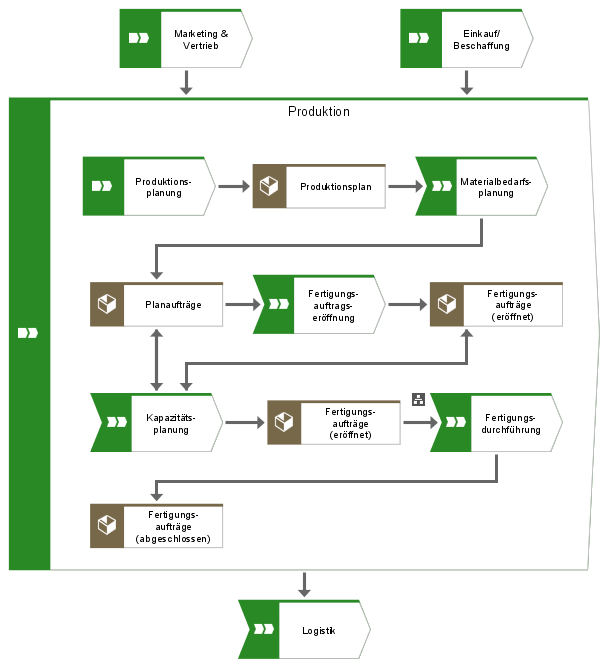
\includegraphics[width=\textwidth]{img/Production_IST.png}	\caption[TEST]{\label{fig:logo}test
	}
\end{figure}


% \begin{figure}[H]
% 	\centering 
% 	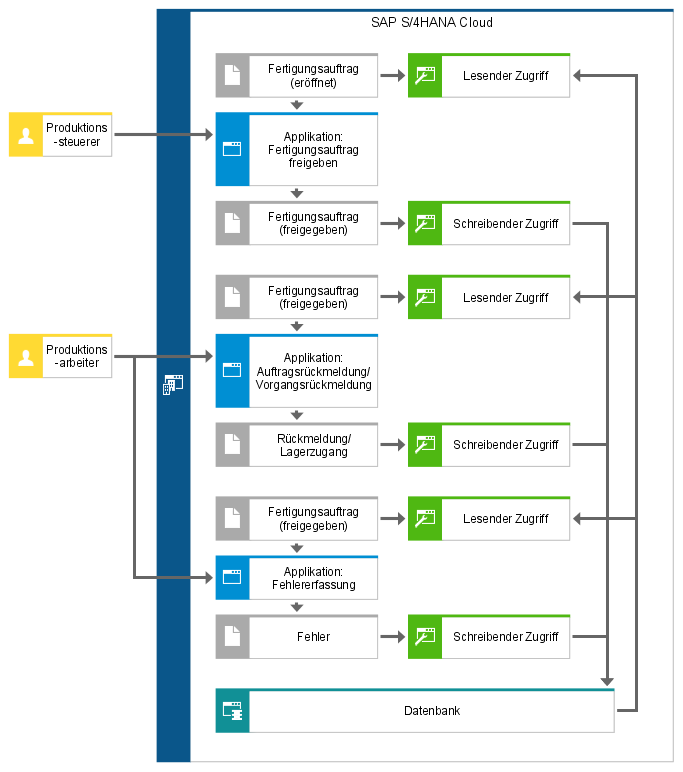
\includegraphics[width=\textwidth]{img/Arch_IST.png}	\caption[TEST]{\label{fig:logo}test
% 	}
% \end{figure}

% \begin{figure}[H]
% 	\centering 
% 	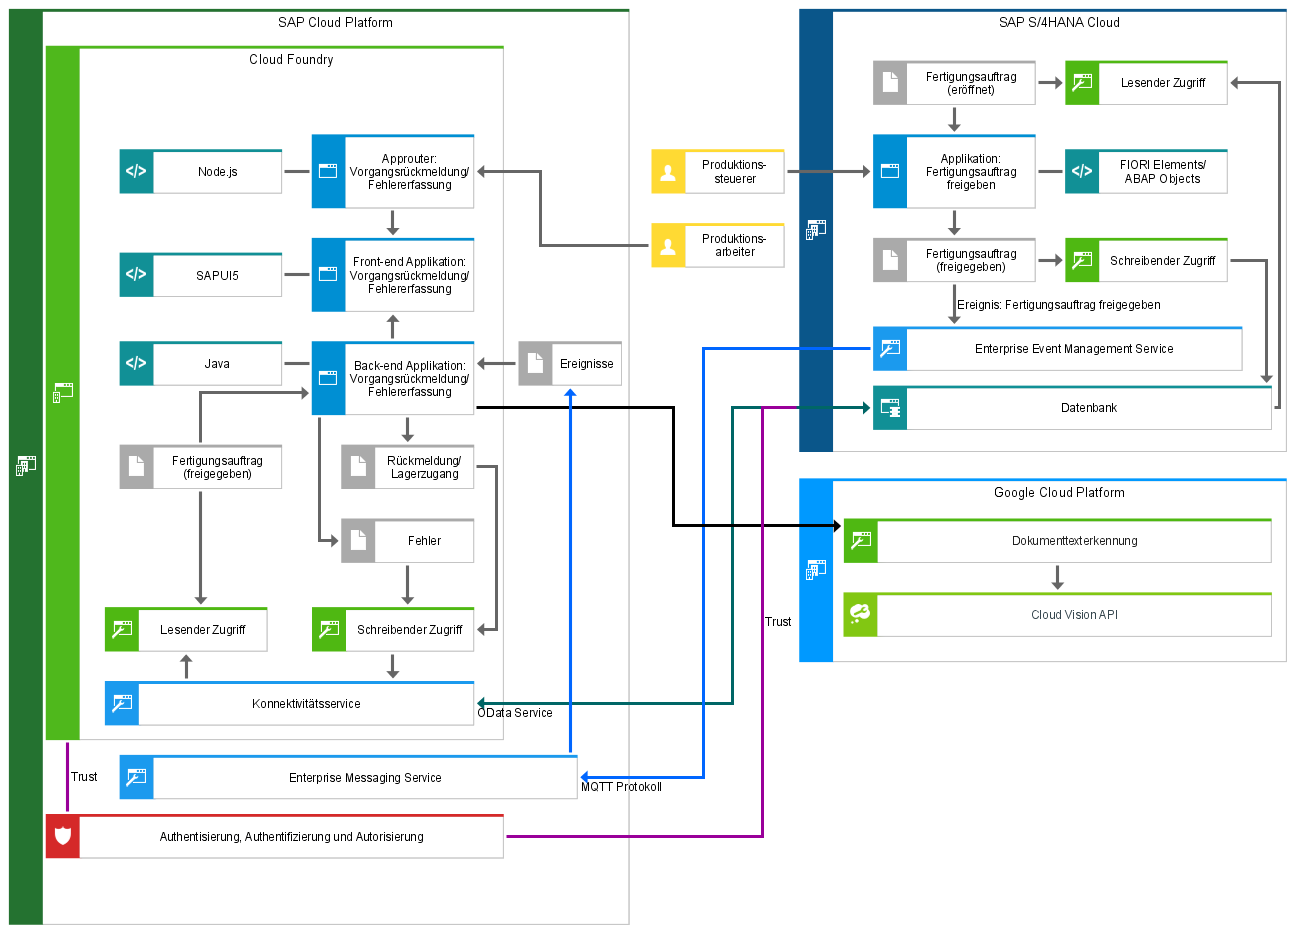
\includegraphics[angle=270,width=\textwidth]{img/Arch_SOLL.png}	\caption[TEST]{\label{fig:logo}test
% 	}
% \end{figure}

% \begin{figure}[H]
% 	\centering 
% 	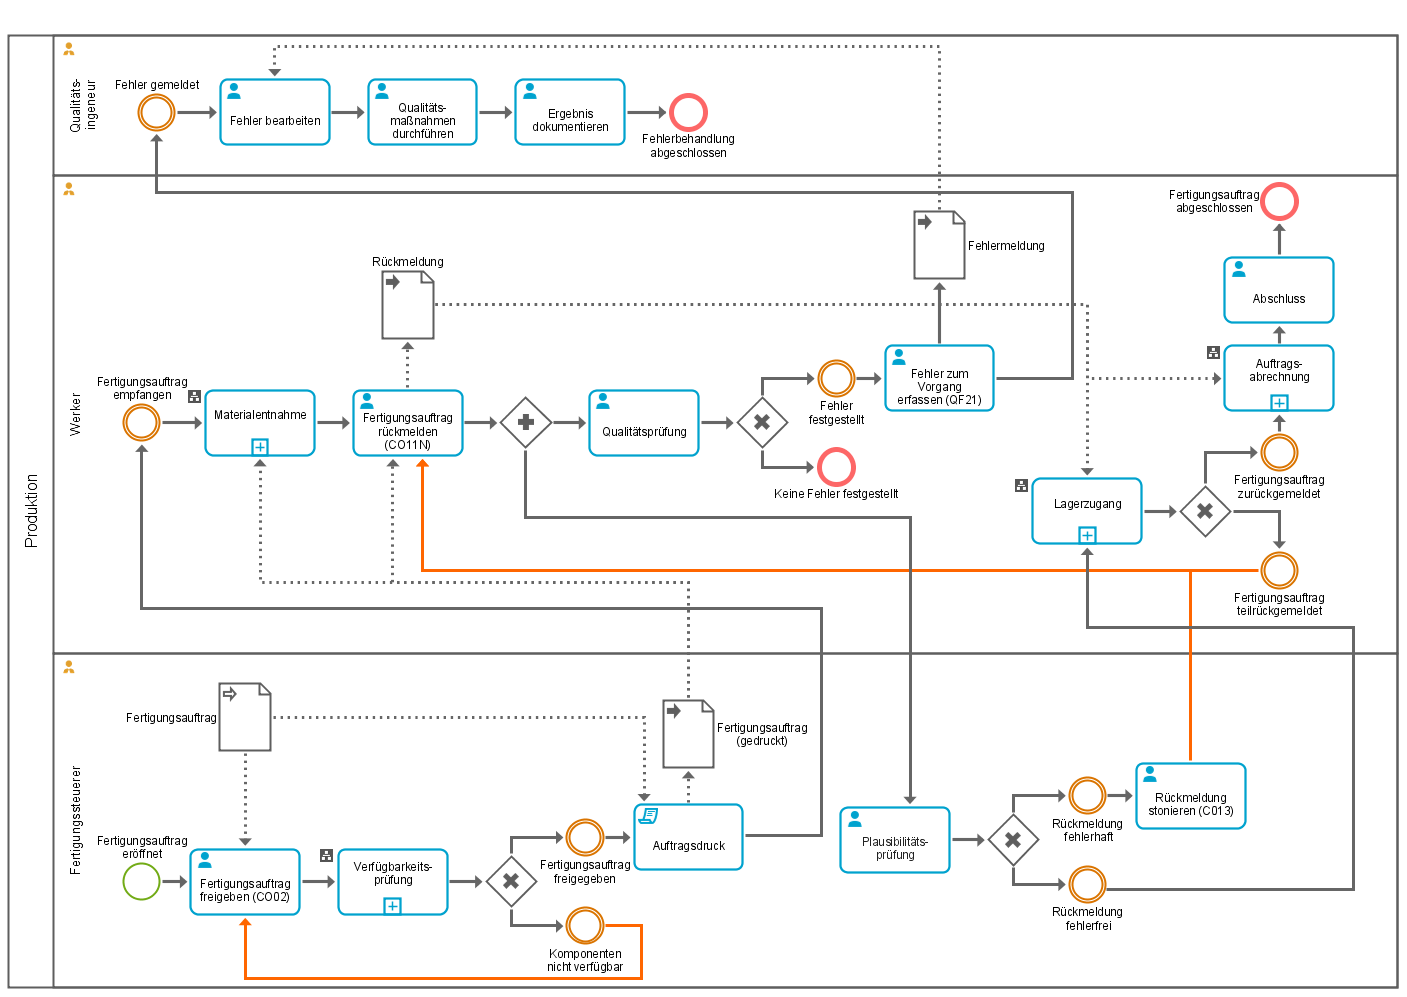
\includegraphics[angle=270,width=\textwidth]{img/Order_Operating_IST.png}	\caption[TEST]{\label{fig:logo}test
% 	}
% \end{figure}

% \begin{figure}[H]
% 	\centering 
% 	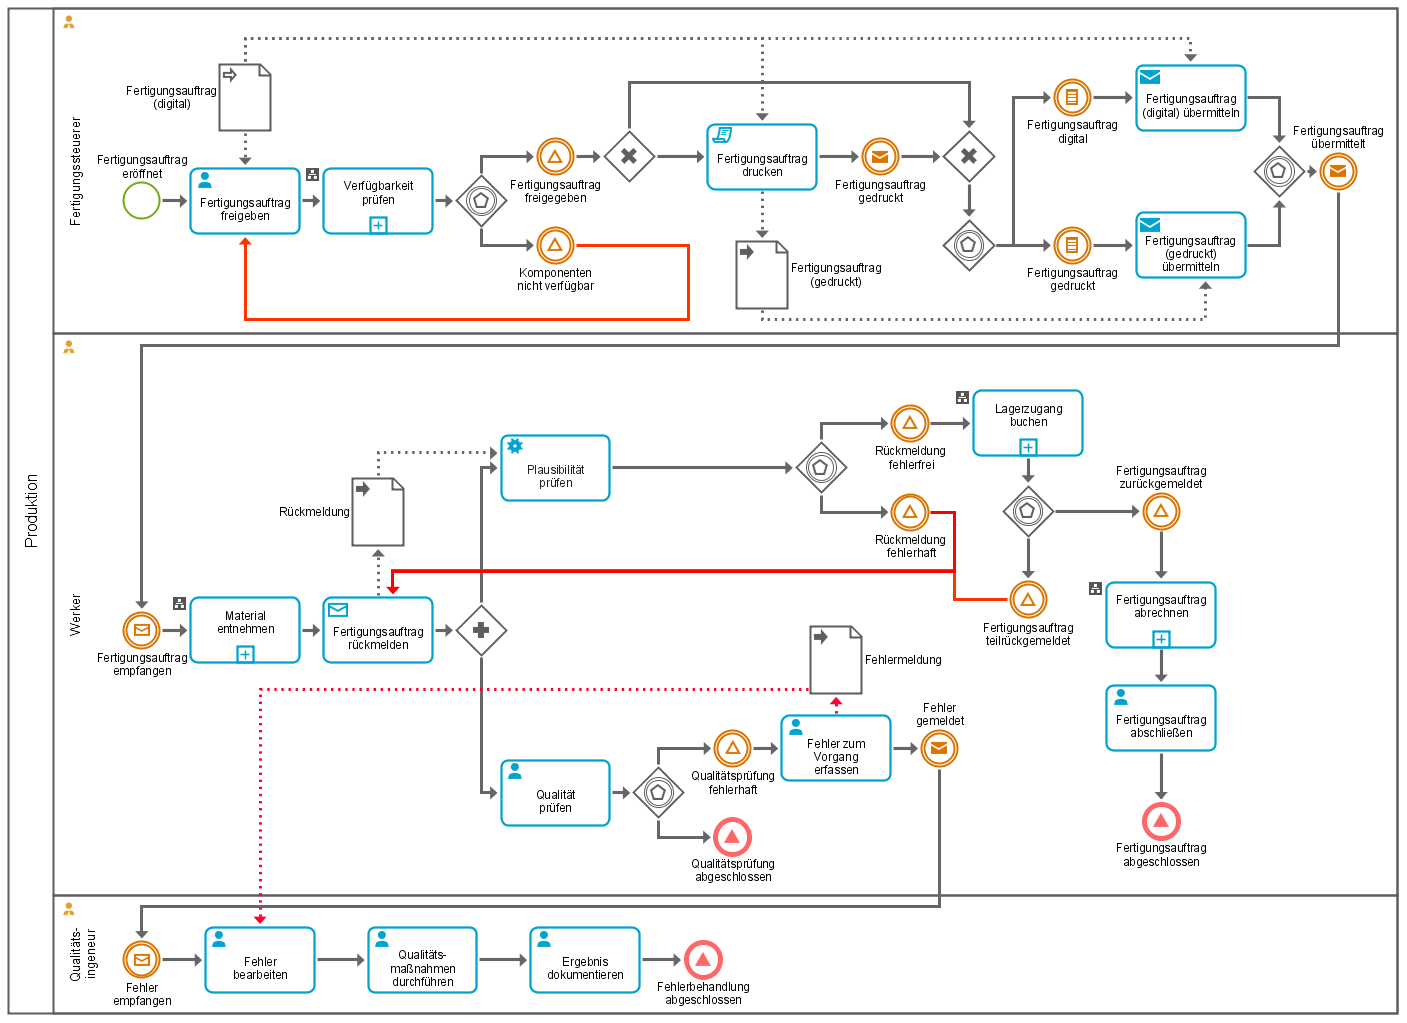
\includegraphics[angle=270,width=\textwidth]{img/Order_Operating_SOLL.png}	\caption[TEST]{\label{fig:logo}test
% 	}
% \end{figure}

% \begin{algorithm}[H]
% \centering 
% \inputminted[linenos]{java}{code/Application.java}
% \caption{Application.java}
% \end{algorithm}

% \begin{algorithm}[H]
% \centering 
% \inputminted[linenos]{java}{code/MessageController.java}
% \caption{MessageController.java}
% \end{algorithm}

% \begin{algorithm}[H]
% \centering 
% \inputminted[linenos]{java}{code/ProductionOrderController.java}
% \caption{ProductionOrderController.java}
% \end{algorithm}

% \begin{algorithm}[H]
% \centering 
% \inputminted[linenos]{java}{code/ProductionOrderReleasedNotificationListener.java}
% \caption{ProductionOrderReleasedNotificationListener.java}
% \end{algorithm}

% \begin{algorithm}[H]
% \centering 
% \inputminted[linenos]{java}{code/EventMessagingService.java}
% \caption{EventMessagingService.java}
% \end{algorithm}

\begin{algorithm}[H]
\centering 
% \lstinputlisting[style=JavaStyle, caption=pr.java]{code/test.java}
\inputminted[linenos]{js}{code/test.js}
\caption{test.js}
\end{algorithm}

% \begin{algorithm}[H]
% \centering 
% % \lstinputlisting[language=ABAP, caption=test.abap]{code/test.abap}
% \inputminted[linenos]{ABAP}{code/RaiseEvent.abap}
% \caption{Exemplarisches Auslösen eines Ereignisses in SAP S/4HANA}
% \end{algorithm}

% \begin{algorithm}[H]
% \centering 
% % \lstinputlisting[language=ABAP, caption=test.abap]{code/test.abap}
% \inputminted[linenos]{js}{code/test.json}
% \caption{Exemplarisches Auslösen eines Ereignisses in SAP S/4HANA}
% \end{algorithm}

\begin{definitionForm}[Definition]
Diese Hervorhebungen können für deine Arbeit an machen stellen sehr nützlich sein. Besonders bei Definitionen macht es einen guten Eindruck, wenn diese in solch einer Form dargestellt ist. 
\end{definitionForm}

DHBW Richtlinie: Laut den aktuellen Angaben der DHBW sind diese Boxen nicht notwendig. Helfen können sie jedoch, um einen Faktor speziell hervorzuheben. Bitte beachte, dass deine Projektarbeit oder auch Bachelorarbeit kein Bilderbuch ist! Alles was eingebunden wird sollte schlicht und dezent dargestellt sein.

\begin{attentionForm}[SOA und Webservices sind nicht grundsätzlich synonym]
An dieser Stelle sei jedoch der Hinweis erlaubt, dass das Konzept der Serviceorientierung allgemeiner ist und schon früher existierte als Webservices. Webservices sollten daher nur als eine, wenn auch zum Verfassungszeitpunkt dieses Buches als wahrscheinlich am besten geeignete Möglichkeit zur Realisierung serviceorientierter Architekturen betrachtet werden.
\end{attentionForm}



\begin{table}[H]
	\centering
	\begin{tabularx}{\textwidth}{|l|X|} 
		\hline
		Auslöser                                     &   
		Der Produktionsplaner möchte Engpässe an betroffenen Arbeitsplätzen durch Modifikationen an Kapazitätsangeboten beheben. \\ 
		\hline\hline
		Input                                         &   
		Handlungsbedarf durch die Auswertung der Kapazitätsauslastung \\ 
		\hline\hline
		Aktivitäten &   
		\begin{minipage}{5in}
    		\begin{enumerate} 
        		\renewcommand{\labelenumi}{(\arabic{enumi})}
        		\item Starten der Anwendung
        		\item Iterative Vorgehensweise bis zur Zielerreichung:
            		\begin{enumerate} 
            		\renewcommand{\labelenumi}{(\arabic{enumi})}
            		\item Wahl einer Arbeitsplatzkapazität
            		\item Erstellung einer Angebotskapazität
            		\item Festlegung eines Gültigkeitszeitraums
            		\item Pflege von Schichten in der Angebotskapazität
            		\item Speichern der Änderungen
            		\end{enumerate}
            	\item Ende des Prozesses
    		\end{enumerate}
    		\vspace{1pt}		
		\end{minipage} \\
		\hline\hline
		Output                                        &   
		Modifizierte Kapazitätsangebote von Arbeitsplätzen  \\
		\hline
	\end{tabularx}
	\caption{\label{tab:aktivitäten}Ist-Prozessbeschreibung }
\end{table}

\begin{table}[H]
	\centering
	\begin{tabularx}{\textwidth}{l X} 
		\toprule
		\textbf{Kriterium}  &   
		\textbf{Beschreibung}  \\ 
		\midrule
		OP1 &   
		Keine Modifikationsmöglichkeiten  \\  \cmidrule(r){1-1} \cmidrule(r){2-2}
		OP2 &   
		Unausgereifter Prozessablauf \\ \cmidrule(r){1-1} \cmidrule(r){2-2}
		OP3 &   
		Mangelhafte Bedienbarkeit  \\ \cmidrule(r){1-1} \cmidrule(r){2-2}
		OP4 &   
		Kontraintuitives Stammdatenmodell  \\ \cmidrule(r){1-1} \cmidrule(r){2-2}
		OP5 &   
		Keine Überprüfung der Validität der Eingaben  \\ \cmidrule(r){1-1} \cmidrule(r){2-2}
		OP6 &   
		Kein Überblick über getätigte Modifikationen  \\
	    \bottomrule
	\end{tabularx}
	\caption{\label{tab:potentiale}Optimierungspotenziale des Ist-Systems}
\end{table}



% \resizebox{\textwidth}{!}{%
% \begin{tikzpicture}

% % Fragestellungs
% \node (goal) [goal] {Entwicklung eines dynamischen Gesch{\"a}ftsprozesses zur ereignisgesteuerten Betriebsdatenerfassung mit SAP S/4HANA Cloud};

% % Wozu?
% \node (wozu) [question, node distance=7cm and 0.5cm, above left=of goal] {Wohin?};
% \draw [] (goal) |- (wozu);


% % Einleitung
% \node (einleitung)[main,draw,rectangle, minimum height = 6cm, node distance=0.5cm and 0.5cm, below=of wozu] {};

% \node (Einleitung) at (einleitung.north) [anchor=north] {\ref{ch:einleitung} \nameref{ch:einleitung}};
% \node (Motivation) [submain,below=of Einleitung] {Motivation}
% \node (Problemstellung) [submain, below=of Motivation] {Problemstellung};
% \node (Zielsetzung) [submain, below=of Problemstellung] {Zielsetzung};
% \node (Vorgehen) [submain, below=of Zielsetzung] {Vorgehen};

% \draw [->] (Motivation) -- (Motivation |- Problemstellung.north); 
% \draw [->] (Problemstellung) -- (Problemstellung |- Zielsetzung.north); 
% \draw [->] (Zielsetzung) -- (Zielsetzung |- Vorgehen.north); 
% % \draw [->] (gui1) -- (gui1 |- pssub1.north); 

% % Was?
% \node (was) [question, node distance=6cm and 0.5cm, above right=of goal] {Was?};
% \draw [] (goal) |- (was);

% % Grundlagen
% \node (grundlagen)[main,draw,rectangle, minimum height = 4cm, node distance=0.5cm and 0.5cm, below=of was] {};

% \node (Grundlagen) at (grundlagen.north) [anchor=north] {\ref{ch:Grundlagen} Stand der Wissenschaft und Technik};
% \node (Automatisierung) [submain,below=of Grundlagen] {Automatisierung von Gesch{\"a}ftsprozessen};
% \node (pssub2) [submain, below=of Automatisierung] {};

% \end{tikzpicture}
% }%


% Ehrenwörtliche Erklärung ewerkl.tex einziehen
% !TEX root =  master.tex

\clearpage
\chapter*{Ehrenwörtliche Erklärung}

% Wird die folgende Zeile auskommentiert, erscheint die ehrenwörtliche
% Erklärung im Inhaltsverzeichnis.

\addcontentsline{toc}{chapter}{Ehrenwörtliche Erklärung}

Ich versichere hiermit, dass ich die vorliegende Arbeit
 mit dem Thema: \textit{\DerTitelDerArbeit} selbstständig verfasst und keine anderen als die angegebenen Quellen und
Hilfsmittel benutzt habe. Ich versichere zudem,
dass die eingereichte elektronische Fassung mit der gedruckten Fassung übereinstimmt.

\vspace{3cm}
Ort, Datum \hfill \DerAutorDerArbeit



\end{document}

